% Biên dịch bằng pdfLaTeX (Overleaf: Menu > Compiler > pdfLaTeX, mặc định), main document: main.tex.
% Dựa trên mẫu báo cáo HUS (extbook 13pt, T5, babel vietnamese, mathptmx).
\PassOptionsToPackage{table}{xcolor}   % cho \rowcolors / \rowcolor trong bảng
\documentclass[13pt, a4paper, oneside]{extbook}

% =========================================================
% THÔNG TIN BÌA (\TODO chỉ còn dùng cho phần của Bích)
% =========================================================
\newcommand{\TODO}[1]{\textcolor{red}{[#1]}}
\newcommand{\MonHoc}{MAT3562E -- Computer Vision}
\newcommand{\GiangVien}{TS. Cao Văn Chung}
\newcommand{\HocKy}{Học kỳ 1, năm học 2026--2027}
\newcommand{\TenA}{Bùi Thuỳ Châu Anh}
\newcommand{\MssvA}{24001963}
\newcommand{\TenB}{Nguyễn Ngọc Bích}
\newcommand{\MssvB}{24001977}

% =========================================================
% GÓI TIẾNG VIỆT, ENCODING & PHÔNG CHỮ
% =========================================================
\usepackage[utf8]{inputenc}
\usepackage[T5]{fontenc}
\usepackage[english, vietnamese]{babel} % Tiếng Việt là ngôn ngữ chính (ngôn ngữ cuối trong danh sách)
\usepackage{vietnam}                    % Giữ gói này từ đoạn 2 để đảm bảo tương thích font
\usepackage{mathptmx}                   % Font Times New Roman
\usepackage{indentfirst}                % Thụt lề đầu dòng ở mọi dòng đầu đoạn

% =========================================================
% LAYOUT, CANH LỀ & TYPOGRAPHY
% =========================================================
\usepackage[
  left=2cm, right=2cm, top=2.5cm, bottom=2.5cm
]{geometry}
\usepackage{setspace}
\onehalfspacing                         % Cách dòng 1.5
\usepackage{microtype}                  % Tối ưu hóa khoảng cách chữ
\usepackage[parfill]{parskip}           % Thêm khoảng cách giữa các đoạn văn

% =========================================================
% TOÁN HỌC & ĐỊNH LÝ
% =========================================================
\usepackage{amsmath}
\usepackage{amssymb}
\usepackage{amsthm}
\usepackage{amsfonts}
\usepackage{amsxtra, latexsym, amscd}
\usepackage{cases}

% =========================================================
% HÌNH ẢNH & ĐỒ HỌA
% =========================================================
\usepackage{graphicx}

\usepackage{float}                      % Hỗ trợ định vị cứng [H] cho hình/bảng
\usepackage{subcaption}                 % Hỗ trợ tạo ảnh con (subfigures)
\usepackage{pdfpages}                   % Cho phép chèn các trang PDF sẵn có
\usepackage{tikz}
\usetikzlibrary{positioning, arrows.meta}
% =========================================================
% BẢNG BIỂU (TABLES)
% =========================================================
\usepackage{booktabs}
\usepackage{tabularx}
\usepackage{longtable}
\usepackage{array}
\usepackage{multirow}
\usepackage{multicol}
\usepackage{colortbl}                   % Đổ màu nền cho các ô trong bảng

\usepackage{xcolor}                     % Định nghĩa màu sắc cho chú thích
\usepackage{dirtree}                    % Vẽ cây thư mục chuyên nghiệp
\renewcommand{\DTstylecomment}{\ttfamily\small\color{gray}} % Làm mờ phần chú thích dấu #

% Định nghĩa màu sắc cho bảng
\definecolor{tableheader}{RGB}{68,114,196}
\definecolor{tablerowalt}{RGB}{235,241,251}

% Khởi tạo Counter tự đánh số bảng (từ đoạn code 1)
\newcounter{tablectr}
\newcommand{\tabletitle}[1]{%
  \stepcounter{tablectr}%
  \noindent\textbf{\thetablectr. #1}%
  \par\vspace{4pt}%
}

% Định nghĩa lại cột căn trái cố định độ rộng cho mảng
\newcolumntype{L}[1]{>{\raggedright\arraybackslash}p{#1}}
% Ô tiêu đề bảng: nền xanh, chữ trắng đậm
\newcommand{\tblhd}[1]{\cellcolor{tableheader}\textcolor{white}{\bfseries #1}}

% =========================================================
% ĐỊNH DẠNG MÃ NGUỒN (CODE LISTINGS) & TCOLORBOX
% =========================================================
\usepackage{listings}
\usepackage{tcolorbox}
\usepackage{xcolor}                     % Định nghĩa màu mở rộng (cho code và tcolorbox)

\lstset{
  basicstyle=\small\ttfamily,
  breaklines=true,
  frame=single,
  backgroundcolor=\color{gray!8},
  keywordstyle=\color{blue}\bfseries,
  commentstyle=\color{green!60!black},
  stringstyle=\color{red!70!black},
  numbers=left,
  numberstyle=\tiny\color{gray},
  stepnumber=1,
  tabsize=4
}

% Tên hàm / cột / tham số: dùng \code{...}, gạch dưới phải viết \_ .
\DeclareRobustCommand{\code}[1]{\texttt{\small #1}}

% =========================================================
% THUẬT TOÁN / GIẢ MÃ (ALGORITHMS)
% =========================================================
\usepackage{algorithm}
\usepackage{algpseudocode}

\makeatletter
% FIX counter cho book class để đánh số từ 1 chạy liên tục
\renewcommand{\thealgorithm}{\arabic{algorithm}}
% Ép cỡ chữ nhỏ cho thuật toán
\renewcommand{\ALG@beginalgorithmic}{\footnotesize}
\makeatother

% Chỉnh cỡ chữ cho số dòng trong thuật toán
\algrenewcommand\alglinenumber[1]{\tiny #1}

% Định nghĩa từ khóa thuật toán sang tiếng Việt
\algrenewcommand\algorithmicrequire{\textbf{Đầu vào:}}
\algrenewcommand\algorithmicensure{\textbf{Đầu ra:}}
\floatname{algorithm}{Thuật toán}

% =========================================================
% DANH SÁCH (LISTS / BULLETS)
% =========================================================
\usepackage{enumitem}
\setlist[itemize]{leftmargin=*, itemsep=2pt}

% =========================================================
% ĐỊNH DẠNG TIÊU ĐỀ, MỤC LỤC & HEADER/FOOTER
% =========================================================
\usepackage{titlesec}
\usepackage{tocloft}
\usepackage{fancyhdr}

\titleformat{\chapter}[block]
  {\normalfont\Large\bfseries\centering}
  {CHƯƠNG \thechapter:}{0.5em}{}
\titlespacing*{\chapter}{0pt}{0pt}{20pt}

\titleformat{\section}
  {\normalfont\large\bfseries}
  {\thesection}{1em}{}
\titleformat{\subsection}
  {\normalfont\large\bfseries}
  {\thesubsection}{1em}{}
\titleformat{\subsubsection}
  {\normalfont\large\itshape}
  {\thesubsubsection}{1em}{}

% =========================================================
% THAM CHIẾU, CHÚ THÍCH & LIÊN KẾT (HYPERLINKS)
% =========================================================
\usepackage{caption}
\captionsetup{font=small, labelfont=bf}

\usepackage{footnote}
\usepackage{placeins}                   % Kiểm soát trôi nổi của ảnh/bảng (\FloatBarrier)
\usepackage{url}
\usepackage{imakeidx}                   % Tạo mục lục tra cứu (Index)

% Thứ tự nạp gói Tài liệu tham khảo và Hyperref rất quan trọng để tránh lỗi link!
\usepackage[sort, numbers]{natbib}
\usepackage[hidelinks]{hyperref}        % Hyperref luôn đặt gần cuối
\usepackage{cleveref}                   % Cleveref PHẢI đặt sau hyperref

\captionsetup{
    font={it}, % In nghiêng
    labelfont={bf},  % Chữ đậm cho "Hình" hoặc "Bảng"
    textfont=it      % Nội dung caption in nghiêng
}

\makeatletter
\def\cleardoublepage{\clearpage\if@twoside \ifodd\c@page\else
    \hbox{}
    \thispagestyle{plain}
    \newpage
    \if@twocolumn\hbox{}\newpage\fi\fi\fi}
\makeatother
\usepackage{boxedminipage,fancybox}
\font\tench=t5-lmb10 at18pt%
\titleformat{\chapter}[display]
{\normalfont\large\filcenter\bfseries}
{{{\chaptertitlename\,}\thechapter}} {1pc}{%\vspace{1pc}%
{\tench}\MakeUppercase}% Dinh nghia lai ten chuong
\renewcommand{\theenumi}{\textbf{\arabic{enumi}}}%Danh lai so thu tu
\renewcommand{\labelenumi}{\theenumi )}%Danh lai so thu tu
\renewcommand{\theequation}{\thechapter.\arabic{equation}}% Danh lai so cong thuc toan
\font\tieude=t5-lmb10 at 14pt
\pagestyle{fancy}
\usepackage{tocloft,calc}
\usepackage{afterpage}
\newcommand\blankpage{%
    \null
    \thispagestyle{plain}%
    \thispagestyle{empty}%
    \newpage}
\setlength{\parindent}{1cm}
\pagestyle{fancy}
\fancyhf{}
\rhead{\bf{Dự án 9}}
\lhead{\bf{\emph{Phát hiện biển số xe và tách ký tự bằng xử lý ảnh cổ điển}}}
\cfoot{\thepage}
\numberwithin{subsection}{section}
%------------------------------------------------------------
\theoremstyle{plain}
\newtheorem{theorem}{Định lý}[section]
\newtheorem{corollary}[theorem]{Hệ quả}
\newtheorem{problem}{Bài toán}
\newtheorem{lemma}[theorem]{Bổ đề}
\newtheorem{proposition}[theorem]{Mệnh đề}
\theoremstyle{definition}
\newtheorem{definition}[theorem]{Định nghĩa}
\newtheorem{example}[theorem]{Ví dụ}
\theoremstyle{remark}
\newtheorem{remark}[theorem]{Nhận xét}

%-----------------------------------------------------------------------
\definecolor{dkgreen}{rgb}{0,0.6,0}
\definecolor{gray}{rgb}{0.5,0.5,0.5}
\definecolor{mauve}{rgb}{0.58,0,0.82}
\usepackage{times}

\begin{document}
\font\chuong=t5-lmb10 at14pt%
\def\chaptername{\chuong Chương}
\renewcommand{\contentsname}{MỤC LỤC}
\renewcommand{\listfigurename}{DANH MỤC HÌNH ẢNH}
\renewcommand{\listtablename}{DANH MỤC BẢNG BIỂU}
\renewcommand{\figurename}{Hình}
\renewcommand{\tablename}{Bảng}
\fontsize{13pt}{13pt}\selectfont% Chon cỡ font

% =========================================================
% TRANG BÌA
% =========================================================
\thispagestyle{empty}
\thisfancypage{\fboxrule=8\fboxrule
	\fboxsep=2\fboxsep
\fbox}{}
\begin{center}
\begin{large}
{\fontsize{13pt}{1}\selectfont ĐẠI HỌC QUỐC GIA HÀ NỘI}
\end{large} \\
\begin{large}
{\fontsize{13pt}{1}\selectfont TRƯỜNG ĐẠI HỌC KHOA HỌC TỰ NHIÊN}
\end{large} \\
\vspace{2 cm}
\begin{figure}[tph]
    \centering
    
\includegraphics[width=4.3cm,height=5.1cm]{image/HUS.png}
\end{figure}
\vspace{1.5cm}
\textbf{BÁO CÁO GIỮA KỲ}
\begin{center}
{\fontsize{18pt}{1}\selectfont\textbf{PHÁT HIỆN BIỂN SỐ XE VÀ TÁCH KÝ TỰ BẰNG XỬ LÝ ẢNH CỔ ĐIỂN}}\\[0.5cm]
{\fontsize{14pt}{1}\selectfont\textbf{(Dự án 9)}}
\end{center}
\vspace{1cm}

\begin{center}
    \textbf{\MonHoc}\\[0.2cm]
    \textbf{\HocKy}\\[1.5cm]

    \begin{tabular}{l l}
        \textbf{Giảng viên:} & \textbf{\GiangVien} \\
                            [0.8cm]
        Nhóm thực hiện: & \TenA\ (\MssvA) \\
                                 & \TenB\ (\MssvB) \\
    \end{tabular}
\end{center}
\vspace{1 cm}
\begin{center}
{\fontsize{14pt}{1}\selectfont \textbf{Hà Nội -- 2026}}
\end{center}
\end{center}
\clearpage
\thispagestyle{plain}

\newpage

% =========================================================
% PHÂN CÔNG NHIỆM VỤ & XÁC NHẬN
% =========================================================
\chapter*{PHÂN CÔNG NHIỆM VỤ}
{\addcontentsline{toc}{chapter}{Phân công nhiệm vụ}}
\baselineskip
25pt
\begin{center}
    \renewcommand{\arraystretch}{1.7}
    \begin{tabular}{|m{10cm}|m{4.5cm}|}
        \hline
        \textbf{Công việc }& \textbf{Người phụ trách} \\
   \hline
   Tiền xử lý, định vị dựa trên biên và HOG-SVM, nắn phối cảnh &  \TenA \\
   \hline
   Đánh giá (evaluate), trực quan hóa, thí nghiệm E2, E3, E4, E7, phân tích lỗi (triage) &  \TenA \\
   \hline
   Phân tích hệ màu (E1), nhị phân hóa (E5), tách ký tự CCA và projection (E6) &  \TenB \\
   \hline
   Khung run\_all và E0, gán nhãn ký tự, ảnh VN định tính (E8) &  \TenB \\
   \hline
   Hoàn thiện, chỉnh sửa báo cáo & Tất cả các thành viên \\
   \hline
   Hoàn thiện chỉnh sửa slide & Tất cả các thành viên \\
        \hline
    \end{tabular}
\end{center}

\newpage

\begin{center}
    \textbf{\Large XÁC NHẬN CỦA CÁC THÀNH VIÊN NHÓM}
\end{center}

\vspace{1.5cm} % Khoảng cách từ tiêu đề xuống bảng

\noindent
\renewcommand{\arraystretch}{3.5} % Tăng độ giãn dòng để có không gian ký tên
\begin{tabular}{@{}p{8cm} l@{}}
    \textbf{Họ và tên} & \textbf{Chữ ký} \\
    \TenA & \rule{6cm}{0.5pt} \\
    \TenB & \rule{6cm}{0.5pt}
\end{tabular}

\newpage

% =========================================================
% MỤC LỤC, DANH MỤC HÌNH, DANH MỤC BẢNG
% =========================================================
\setcounter{tocdepth}{1} % Mục lục hiển thị đến cấp section
\baselineskip 0.6cm
\tableofcontents
\newpage
\setlength{\cftfignumwidth}{1.8cm}
\setlength{\cfttabnumwidth}{1.8cm}
\renewcommand{\cftfigpresnum}{Hình~}
\renewcommand{\cfttabpresnum}{Bảng~}
\listoffigures
\newpage
\listoftables
\newpage

% =========================================================
% NỘI DUNG
% =========================================================
\chapter{GIỚI THIỆU BÀI TOÁN, DỮ LIỆU VÀ ĐỘ ĐO}
\label{chap:intro}

\section{Bài toán}
\label{sec:problem}

Bài toán được đặt trong ngữ cảnh một hệ thống kiểm soát xe ra vào bãi gửi xe. Camera cố định chụp xe; hệ thống cần định vị biển số, nắn biển về hình chữ nhật chuẩn, rồi tách từng ký tự để chuẩn bị cho bước nhận dạng ký tự (OCR) về sau. Với mỗi ảnh đầu vào, đầu ra giữa kỳ gồm hộp biển số, ảnh biển đã nắn và danh sách hộp ký tự.

Dự án chỉ dùng xử lý ảnh cổ điển, không dùng học sâu. Các nội dung nằm ngoài phạm vi giữa kỳ là nhận dạng ký tự, mô hình học sâu, giao diện web, và biển hai dòng trong đánh giá định lượng. Pipeline gồm các bước: tiền xử lý, định vị biển, nắn phối cảnh, nhị phân hóa và tách ký tự. Nhóm có hai thành viên: thành viên A (Châu Anh) phụ trách ba bước đầu và phần đánh giá, thành viên B (Bích) phụ trách hệ màu, nhị phân hóa và tách ký tự (xem bảng phân công ở đầu báo cáo).

\section{Dữ liệu}
\label{sec:data}

Dữ liệu là một tập con của CCPD2019 \cite{ccpd} gồm 660 ảnh có biển xanh Trung Quốc 7 ký tự: nhóm \code{base} 500 ảnh và bốn nhóm khó \code{tilt}, \code{blur}, \code{db} (ngược sáng hoặc chói), \code{challenge}, mỗi nhóm 40 ảnh. Chỉ lấy ảnh có chuỗi biển hợp lệ (đủ 7 ký tự). Mỗi ảnh có đúng một biển. Việc lấy mẫu dùng seed 42.

Ngoài ra có 40 ảnh biển số Việt Nam tự chụp (làm mờ mặt người trước khi đưa vào kho mã), chỉ dùng cho đánh giá định tính (thí nghiệm E8, phần của B). Các ảnh này không dùng để chỉnh ngưỡng, không dùng làm mẫu huấn luyện và không tính vào bảng số liệu, vì phần lớn là biển xe máy hai dòng gần vuông, khác hẳn phân bố của CCPD.

\section{Chia tập tune và test}
\label{sec:split}

Ảnh được chia cố định (seed 42), phân tầng theo nhóm, thành tập \emph{tune} (30\%, 198 ảnh) dùng để chọn tham số và huấn luyện, và tập \emph{test} (70\%, 462 ảnh) chỉ dùng để báo cáo (Bảng~\ref{tab:split}).

\begin{table}[htbp]
\centering
\caption{Chia tập dữ liệu (số ảnh).}
\label{tab:split}
\small
\rowcolors{2}{white}{tablerowalt}
\begin{tabular}{lrrrrrr}
\toprule
\rowcolor{tableheader} \tblhd{} & \tblhd{base} & \tblhd{tilt} & \tblhd{blur} & \tblhd{db} & \tblhd{challenge} & \tblhd{Tổng} \\
\midrule
tune & 150 & 12 & 12 & 12 & 12 & 198 \\
test & 350 & 28 & 28 & 28 & 28 & 462 \\
\bottomrule
\end{tabular}
\end{table}

\textbf{Kỷ luật tune và test.} Mọi tham số và lựa chọn phương pháp được chọn chỉ dựa trên tập tune: bộ lọc ở E2 và phương pháp ở E3 được chọn theo F1 trên toàn tune, hòa thì theo thứ tự cố định; SVM chỉ huấn luyện trên tune; ngưỡng chia lỗi ở mục triage tính trên tune. Tập test chỉ dùng để báo cáo, không chỉnh lại tham số sau khi xem số test.

\section{Độ đo}
\label{sec:metrics}

\textbf{Định vị.} Với hai bbox $A$, $B$: $\mathrm{IoU}=|A\cap B|/|A\cup B|$. Mỗi ảnh có một biển và ta lấy ứng viên điểm cao nhất (top-1). Ảnh là TP nếu IoU của top-1 với bbox thật $\geq 0.5$; FP nếu có dự đoán nhưng IoU $<0.5$; FN nếu IoU $<0.5$ hoặc không có ứng viên nào. Khi đó
\[
P=\frac{TP}{TP+FP},\qquad R=\frac{TP}{TP+FN},\qquad F_1=\frac{2PR}{P+R}.
\]
Vì mỗi ảnh có đúng một biển nên $R$ chính là Recall@1. \textbf{Recall@$k$} là tỉ lệ ảnh có ít nhất một ứng viên trong $k$ ứng viên đầu với IoU $\geq 0.5$; Recall@5 cũng là \code{cand\_recall} (trần mà bước xếp hạng có thể đạt), giúp tách lỗi ``không sinh ra ứng viên đúng'' khỏi lỗi ``xếp hạng sai''.

\textbf{Nắn biển.} Sai số góc (\code{corner\_error}) là khoảng cách Euclid trung bình giữa bốn góc tương ứng của quad dự đoán và quad thật, tính bằng pixel của ảnh gốc, chỉ tính trên ảnh định vị đúng (top-1 có IoU $\geq 0.5$). Với phương án cắt bbox, quad ngầm định là bốn góc của bbox dự đoán.

\textbf{Chất lượng tách ký tự (dùng trong E4).} Theo định nghĩa của dự án (do B phụ trách phần tách): \code{count\_match} là tỉ lệ ảnh có đủ 7 hộp ký tự; \code{pos0} là tỉ lệ biển có ký tự Hán (vị trí 0) trúng khuôn vị trí chuẩn; \code{pos1\textendash 6} là tỉ lệ trung bình các vị trí 1 đến 6 trúng khuôn; \code{all\_correct} là đồng thời đủ 7 hộp và cả 7 vị trí đúng. E4 báo ba nguồn crop: \code{gt} (crop từ bbox hoặc quad thật, tách riêng lỗi của bộ tách), \code{pred} (crop từ top-1 trên mọi ảnh, định vị sai tính là hỏng) và \code{pred\_tp} (chỉ các ảnh top-1 đúng).

\section{Bố cục báo cáo}

Chương~\ref{chap:a-method} trình bày phương pháp của thành viên A, Chương~\ref{chap:a-results} báo cáo kết quả các thí nghiệm E2, E3, E4 và E7, Chương~\ref{chap:a-discussion} phân tích lỗi theo bước pipeline, các hạn chế và hướng cải thiện. Chương~\ref{chap:b} dành cho phần của thành viên B (E1, E5, E6, E8). Chương cuối là kết luận.

\chapter{PHƯƠNG PHÁP: TIỀN XỬ LÝ, ĐỊNH VỊ, NẮN PHỐI CẢNH}
\label{chap:a-method}

Chương này mô tả các bước do thành viên A phụ trách: tiền xử lý ảnh, định vị biển số bằng đặc trưng cạnh và hình thái học, chấm điểm lại ứng viên bằng HOG và SVM tuyến tính, và nắn biển về hình chữ nhật chuẩn bằng phép biến đổi phối cảnh. Dữ liệu, cách chia tập và các độ đo dùng cho phần kết quả được trình bày ở Chương~\ref{chap:intro}. Hai bước sau của pipeline (nhị phân hóa và tách ký tự) do thành viên B trình bày (Chương~\ref{chap:b}).

\section{Luồng xử lý}
\label{sec:flow}

Dự án chỉ dùng xử lý ảnh cổ điển, không dùng học sâu. Luồng xử lý một ảnh được tóm tắt ở Hình~\ref{fig:pipeline}. Phương pháp A dùng trực tiếp ứng viên có điểm heuristic cao nhất; phương pháp A+SVM xếp lại tối đa 5 ứng viên theo điểm của SVM rồi lấy ứng viên đầu. Biển được nắn về ảnh $220\times 70$ trước khi sang phần B (Chương~\ref{chap:b}).

\begin{figure}[htbp]
\centering
\begin{tikzpicture}[
  node distance=5mm and 7mm,
  box/.style={draw, rounded corners=2pt, align=center, minimum height=11mm, text width=27mm, font=\fontsize{7pt}{8pt}\selectfont},
  boxB/.style={draw, dashed, rounded corners=2pt, align=center, minimum height=11mm, text width=27mm, font=\fontsize{7pt}{8pt}\selectfont},
  arr/.style={-{Stealth[length=2mm]}, thick}]
  \node[box] (in) {Ảnh xe (BGR)};
  \node[box, right=of in] (pre) {Tiền xử lý\\resize rộng 800, xám,\\CLAHE, lọc nhiễu};
  \node[box, right=of pre] (edge) {Định vị theo cạnh\\Sobel-x, Otsu, close/open,\\contour, lọc, NMS};
  \node[box, right=of edge] (svm) {HOG + SVM\\(chỉ A+SVM)\\xếp lại top-5};
  \node[box, below=of svm] (top1) {Chọn ứng viên top-1\\(bbox + quad)};
  \node[box, left=of top1] (quad) {Ước lượng quad\\approxPolyDP trên\\mặt nạ xanh};
  \node[box, left=of quad] (warp) {Homography\\về ảnh $220\times 70$};
  \node[boxB, left=of warp] (partb) {Phần B\\nhị phân hóa,\\tách ký tự};
  \draw[arr] (in) -- (pre);
  \draw[arr] (pre) -- (edge);
  \draw[arr] (edge) -- (svm);
  \draw[arr] (svm) -- (top1);
  \draw[arr] (top1) -- (quad);
  \draw[arr] (quad) -- (warp);
  \draw[arr] (warp) -- (partb);
\end{tikzpicture}
\caption[Pipeline phần A]{Pipeline phần A. Phương pháp A đi thẳng từ khối định vị sang chọn top-1, bỏ qua khối HOG + SVM.}
\label{fig:pipeline}
\end{figure}

\section{Tiền xử lý}
\label{sec:preprocess}

Ảnh gốc được đưa về chiều rộng 800 pixel, giữ tỉ lệ (nội suy diện tích khi thu nhỏ, tuyến tính khi phóng to), rồi đổi sang ảnh xám. Sau đó áp dụng CLAHE \cite{clahe} (giới hạn tương phản 2.0, lưới $8\times 8$) để cân bằng sáng cục bộ, và cuối cùng là một bộ khử nhiễu. Bốn bộ lọc được so sánh ở thí nghiệm E2:
\begin{itemize}
  \item \code{none}: không lọc;
  \item \code{gaussian}: Gauss, kernel $5\times 5$;
  \item \code{median}: trung vị, kernel $5\times 5$;
  \item \code{bilateral}: song phương \cite{bilateral}, đường kính 11, $\sigma_{\text{color}}=17$, $\sigma_{\text{space}}=17$. Bộ lọc này làm mịn vùng phẳng nhưng giữ cạnh có chênh lệch độ sáng lớn.
\end{itemize}
Mọi tham số của bước định vị phía sau (kernel hình thái, ngưỡng diện tích) tính theo ảnh đã resize về 800 pixel nên không phụ thuộc kích thước ảnh gốc.

\section{Định vị dựa trên cạnh (phương pháp A)}
\label{sec:edge}

Ý tưởng: vùng biển số chứa nhiều nét đứng dày đặc (cạnh các ký tự), nên đạo hàm theo trục $x$ lớn tập trung ở một vùng chữ nhật nằm ngang. Các bước:
\begin{enumerate}
  \item \textbf{Cạnh.} Tính $|G_x|$ bằng Sobel theo $x$ (kernel 3), chuẩn hóa về $[0,255]$ rồi nhị phân hóa bằng Otsu \cite{otsu}.
  \item \textbf{Hình thái học.} Phép \emph{close} với kernel chữ nhật nằm ngang ($21\times 5$, rộng $\times$ cao) để nối các nét ký tự thành một khối, sau đó phép \emph{open} $3\times 3$ để bỏ nhiễu nhỏ.
  \item \textbf{Đa tỉ lệ.} Lặp lại bước close/open với hai kernel phụ $13\times 3$ và $33\times 7$. Biển bị vỡ thành mảnh ở kernel này có thể liền khối ở kernel khác. Ở mỗi kernel, ứng viên được lọc, chấm điểm heuristic và cắt xuống $k=5$ ứng viên cao nhất \emph{trước} khi gộp; sau đó ứng viên của ba kernel được gộp chung, NMS trên bbox (ngưỡng IoU 0.5, giữ điểm cao hơn) và giữ lại $k=5$ ứng viên cao nhất.
  \item \textbf{Ứng viên.} Với mỗi contour ngoài của mặt nạ, lấy hình chữ nhật xoay nhỏ nhất (\code{minAreaRect}); bbox ngang là hình bao của nó, quad là bốn đỉnh sắp theo thứ tự trên-trái, trên-phải, dưới-phải, dưới-trái.
  \item {\sloppy \textbf{Lọc theo đặc trưng hình học.} Với mỗi ứng viên tính: tỉ lệ cạnh dài/ngắn (\code{aspect}), diện tích hình chữ nhật so với diện tích ảnh (\code{area\_ratio}), tỉ lệ pixel mặt nạ trong hình chữ nhật (\code{fill\_ratio}), tỉ lệ pixel cạnh nhị phân trong hình chữ nhật (\code{edge\_density}) và góc nghiêng. Giữ ứng viên thỏa các ngưỡng ở Bảng~\ref{tab:edgeparams}.\par}
  \item \textbf{Điểm heuristic.} Điểm của ứng viên là
  \begin{equation}
    s = 0.4\,d + 0.3\,f + 0.3\exp\!\left(-\frac{\ln^2(a/3.14)}{2\cdot 0.3^2}\right),
  \end{equation}
  trong đó $d$ là \code{edge\_density}, $f$ là \code{fill\_ratio}, $a$ là \code{aspect}; số hạng cuối bằng 1 khi $a\approx 440/140\approx 3.14$, đúng tỉ lệ biển xanh. Giữ tối đa $k=5$ ứng viên điểm cao nhất, quy đổi tọa độ về ảnh gốc bằng cách chia cho hệ số resize.
\end{enumerate}

\begin{table}[htbp]
\centering
\caption{Tham số của bước định vị dựa trên cạnh (cấu hình chốt, tính trên ảnh rộng 800 px).}
\label{tab:edgeparams}
\small
\rowcolors{2}{white}{tablerowalt}
\arrayrulecolor{tableheader}
\begin{tabularx}{\textwidth}{lY}
\hline
\rowcolor{tableheader} \tblhd{Tham số} & \tblhd{Giá trị} \\
\hline
Sobel & theo $x$, kernel 3 \\
close chính / phụ (rộng $\times$ cao) & $21\times 5$ / $13\times 3$, $33\times 7$ \\
open & $3\times 3$ \\
NMS IoU (bbox) & 0.5 \\
\code{aspect} & $[1.5,\ 7.0]$ \\
\code{area\_ratio} & $[0.008,\ 0.16]$ \\
\code{fill\_ratio} tối thiểu & 0.4 \\
\code{edge\_density} tối thiểu & 0.12 \\
Góc nghiêng tối đa & $30^\circ$ \\
Số ứng viên giữ lại $k$ & 5 \\
\hline
\end{tabularx}
\end{table}

Thuật toán~\ref{alg:edge} tóm tắt toàn bộ bước định vị theo cạnh.

\begin{algorithm}[htbp]
\caption{Định vị biển dựa trên cạnh (phương pháp A)}
\label{alg:edge}
\begin{algorithmic}[1]
\Require Ảnh xám đã tiền xử lý $I$ (rộng 800 px), số ứng viên giữ lại $k=5$
\Ensure Tối đa $k$ ứng viên (bbox, quad, điểm), sắp theo điểm giảm dần
\State $G \gets |\textsc{Sobel}_x(I)|$ chuẩn hóa về $[0,255]$;\ $M_0 \gets \textsc{Otsu}(G)$
\State $C \gets \emptyset$
\ForAll{kernel close $K \in \{21\times 5,\ 13\times 3,\ 33\times 7\}$}
    \State $M \gets \textsc{Open}_{3\times 3}\big(\textsc{Close}_K(M_0)\big)$
    \State $C_K \gets \emptyset$
    \ForAll{contour ngoài của $M$}
        \State $r \gets \textsc{MinAreaRect}$;\ tính \code{aspect}, \code{area\_ratio}, \code{fill\_ratio}, \code{edge\_density}, góc
        \If{$r$ thỏa các ngưỡng ở Bảng~\ref{tab:edgeparams}}
            \State thêm $r$ vào $C_K$ với điểm heuristic $s$
        \EndIf
    \EndFor
    \State $C \gets C \cup \textsc{TopK}(C_K, k)$
\EndFor
\State $C \gets \textsc{NMS}(C,\ \text{IoU}=0.5)$;\ $C \gets \textsc{TopK}(C, k)$
\State quy đổi tọa độ về ảnh gốc (chia cho hệ số resize);\ \Return $C$
\end{algorithmic}
\end{algorithm}

Các ngưỡng này được chọn bằng cách quét trên tập tune (mục~\ref{sec:tuning}). Riêng cận dưới của \code{area\_ratio} bám theo phân bố diện tích bbox thật trên tune (phân vị 5\% là 0.0116, lớn nhất 0.153), nhằm loại logo và chữ nhỏ.

\section{Chấm điểm lại ứng viên bằng HOG và SVM (A+SVM)}
\label{sec:hogsvm}

Điểm heuristic chỉ gồm mật độ cạnh, độ lấp đầy và tỉ lệ cạnh nên dễ xếp nhầm chữ hãng xe hay logo lên trên biển thật. Bước này thay điểm đó bằng điểm của bộ phân loại học từ ảnh:
\begin{itemize}
  \item \textbf{Đặc trưng.} Cắt bbox của ứng viên trên ảnh xám, resize về $128\times 32$ (rộng $\times$ cao), trích HOG \cite{hog}: 9 hướng, ô $8\times 8$ pixel, khối $2\times 2$ ô, chuẩn hóa L2-Hys, vector $D=1620$ chiều.
  \item \textbf{Mẫu dương.} Crop bbox thật của 198 ảnh tune.
  \item \textbf{Mẫu âm.} Với mỗi mẫu dương lấy 3 mẫu âm: ưu tiên ứng viên sai của \code{localize\_edge} có IoU với bbox thật dưới 0.3, nếu thiếu thì bù bằng vùng ngẫu nhiên (rộng 8--45\% chiều rộng ảnh, tỉ lệ cạnh trong \code{aspect}, IoU dưới 0.3). Tổng cộng 198 dương và 594 âm.
  \item \textbf{Bộ phân loại.} SVM tuyến tính \cite{svm} (\code{LinearSVC}, $C=1$, seed 42). Điểm của ứng viên là giá trị hàm quyết định; các ứng viên được sắp giảm dần theo điểm này. Không dùng ngưỡng điểm để loại ứng viên, nhằm tính được Recall@$k$.
  \item \textbf{Kiểm chứng chéo.} 5 fold phân tầng trên tập mẫu của tune để ước lượng chất lượng phân loại patch.
\end{itemize}
Thuật toán~\ref{alg:svm} tóm tắt huấn luyện và chấm điểm lại.

\begin{algorithm}[htbp]
\caption{Huấn luyện SVM và xếp lại ứng viên (A+SVM)}
\label{alg:svm}
\begin{algorithmic}[1]
\Require Ảnh tune (198 ảnh) kèm bbox thật; tối đa $k=5$ ứng viên của \code{localize\_edge} cho ảnh cần xử lý
\Ensure Danh sách ứng viên sắp theo điểm SVM giảm dần
\Procedure{Train}{}
    \ForAll{ảnh tune}
        \State mẫu dương: crop bbox thật, resize $128\times 32$, trích HOG ($D=1620$)
        \State 3 mẫu âm: ứng viên sai có IoU $<0.3$, thiếu thì bù vùng ngẫu nhiên có IoU $<0.3$
    \EndFor
    \State huấn luyện \code{LinearSVC} ($C=1$, seed 42) trên 198 dương và 594 âm
\EndProcedure
\Procedure{Rerank}{ứng viên}
    \ForAll{ứng viên}
        \State điểm $\gets$ giá trị hàm quyết định SVM trên HOG của crop bbox ($128\times 32$)
    \EndFor
    \State \Return ứng viên sắp theo điểm giảm dần (không loại ứng viên nào)
\EndProcedure
\end{algorithmic}
\end{algorithm}

SVM chỉ xếp lại tối đa 5 ứng viên mà bước cạnh đã sinh ra, nên nó không thể cứu ảnh mà bước cạnh không sinh ứng viên đúng. Mô hình chỉ huấn luyện trên tune; mã nguồn từ chối dữ liệu không thuộc tune.

\section{Nắn phối cảnh}
\label{sec:rectify}

Ứng viên top-1 cho một bbox ngang và một quad. Biển nghiêng hoặc chụp xiên có quad không phải hình chữ nhật ngang, nên cắt bbox giữ lại nền và làm ký tự méo. Phép nắn đưa biển về ảnh chuẩn $220\times 70$ (tỉ lệ $\approx 3.14$, khớp biển xanh $440\times 140$ mm). Có hai cách lấy quad:
\begin{itemize}
  \item \code{minarearect}: dùng luôn bốn đỉnh \code{minAreaRect} của ứng viên;
  \item \code{approxpoly} (mặc định): tinh chỉnh bốn góc từ màu biển. Trong bbox nới thêm 15\%, tạo mặt nạ màu xanh dương trong HSV ($H\in[95,135]$, $S\ge 70$, $V\ge 40$), đóng và mở hình thái, giới hạn mặt nạ trong quad ứng viên (tránh rò sang nền xanh), lấy contour lớn nhất chứa tâm bbox, bao lồi, rồi \code{approxPolyDP} với $\varepsilon$ tăng từ 1\% đến 15\% chu vi (bước 0.5\%) tới khi còn đúng 4 đỉnh (dừng sớm nếu số đỉnh đã tụt xuống dưới 4). Nếu không ra 4 đỉnh, quad không lồi hoặc diện tích ngoài khoảng $30\%$--$300\%$ diện tích bbox thì lùi về quad \code{minAreaRect}.
\end{itemize}
Với bốn góc nguồn $\mathbf{p}_i$ (sắp theo thứ tự trên-trái, trên-phải, dưới-phải, dưới-trái) và bốn góc đích $(0,0)$, $(219,0)$, $(219,69)$, $(0,69)$, ma trận homography $H\in\mathbb{R}^{3\times 3}$ thỏa $\tilde{\mathbf{x}}'\sim H\tilde{\mathbf{x}}$ (tọa độ thuần nhất) được giải từ bốn cặp điểm, rồi áp dụng nội suy tuyến tính, viền lặp pixel biên. Phương án đối chứng là cắt bbox ngang rồi resize về $220\times 70$ (\code{bbox}), không bù được độ nghiêng.


\chapter{KẾT QUẢ THỰC NGHIỆM}
\label{chap:a-results}

\section{Thiết lập}

Mọi số liệu dưới đây dùng ngưỡng IoU $\ge 0.5$. Tham số và lựa chọn phương pháp được chọn trên tập tune (198 ảnh); các bảng chính báo trên tập test (462 ảnh) và chỉ đo cho cấu hình đã chốt. Các nhóm khó (\code{blur}, \code{db}, \code{challenge}, \code{tilt}) chỉ có 12 ảnh ở tune và 28 ảnh ở test, nên một ảnh đổi kết quả làm tỉ lệ thay đổi $1/28\approx 0.036$; chênh lệch nhỏ ở các nhóm này không nên đọc là xu hướng. Thời gian chạy (ms/ảnh) trong mục này và mục~\ref{sec:e7} đo trên một lần chạy một tiến trình, máy ít tải hơn so với các lần chạy ghi trong sổ thí nghiệm (khi đó nhiều tiến trình khác chạy cùng lúc, số tuyệt đối cao gấp khoảng ba lần); vì vậy chỉ nên so sánh tương đối giữa các dòng của cùng một bảng. Số đo lại trên máy ít tải được ghi ở mục ``Đo lại thời gian (máy ít tải)'', ngày 2026-11-11, trong sổ thí nghiệm \code{notes.md}; bảng trong báo cáo dùng đúng các số đó.

\section{Tiền xử lý: kích thước ảnh và bộ lọc nhiễu (E2)}
\label{sec:e2}

\textbf{Kích thước ảnh.} Ở giai đoạn đầu (tập tune, cấu hình định vị cũ), thử ba chiều rộng resize cho thấy ảnh càng lớn càng tốt (Bảng~\ref{tab:resize}); giữ 800.

\begin{table}[htbp]
\centering
\caption[Ảnh hưởng của chiều rộng resize (tune)]{Ảnh hưởng của chiều rộng resize (tune, $n=198$, cấu hình định vị giai đoạn đầu; nguồn: sổ thí nghiệm, mục Tiền xử lý).}
\label{tab:resize}
\small
\rowcolors{2}{white}{tablerowalt}
\arrayrulecolor{tableheader}
\begin{tabularx}{\textwidth}{lCCCC}
\hline
\rowcolor{tableheader} \tblhd{Chiều rộng} & \tblhd{P} & \tblhd{R} & \tblhd{F1} & \tblhd{R@5} \\
\hline
640 & 0.639 & 0.591 & 0.614 & 0.727 \\
720 (không đổi tỉ lệ) & 0.640 & 0.601 & 0.620 & 0.758 \\
\textbf{800 (chọn, phóng to)} & 0.647 & 0.621 & 0.634 & 0.778 \\
\hline
\end{tabularx}
\end{table}

\textbf{Bộ lọc nhiễu.} E2 chạy \code{localize\_edge} với bốn bộ lọc và cấu hình chốt của mục~\ref{sec:tuning}, trên cả tune và test (Bảng~\ref{tab:e2}). Bộ lọc được chọn chỉ theo F1 trên tune.

\begin{tabular}{llrrrrrr}
\toprule
Tập & Bộ lọc & $n$ & P & R & F1 & R@5 & ms/ảnh \\
\midrule
tune & \textbf{bilateral} & 198 & 0.775 & 0.748 & 0.761 & 0.828 & 132.5 \\
tune & gaussian & 198 & 0.630 & 0.601 & 0.615 & 0.682 & 95.0 \\
tune & median & 198 & 0.637 & 0.611 & 0.624 & 0.697 & 107.7 \\
tune & none & 198 & 0.598 & 0.571 & 0.584 & 0.657 & 97.4 \\
\midrule
test & \textbf{bilateral} & 462 & 0.729 & 0.682 & 0.705 & 0.792 & 111.1 \\
test & gaussian & 462 & 0.647 & 0.615 & 0.630 & 0.712 & 82.4 \\
test & median & 462 & 0.616 & 0.584 & 0.600 & 0.699 & 93.2 \\
test & none & 462 & 0.610 & 0.576 & 0.592 & 0.645 & 84.7 \\
\bottomrule
\end{tabular}


Bilateral cho F1 cao hơn rõ rệt trên cả hai tập: 0.761 so với 0.584--0.624 trên tune và 0.705 so với 0.592--0.630 trên test. Ba bộ lọc còn lại cho kết quả gần nhau, và trên test bộ lọc trung vị (0.600) chỉ nhỉnh hơn \code{none} (0.592) rất ít. Nguyên nhân có thể là bilateral làm mịn nhiễu và các chi tiết nền mà vẫn giữ cạnh nét ký tự, nên bản đồ cạnh Sobel ít ứng viên rác hơn (đây là giả thuyết, chưa kiểm tra riêng). Cái giá là thời gian: bilateral chậm hơn các bộ lọc khác khoảng 18--29 ms/ảnh trong lần đo này (111 ms so với 82--93 ms trên test). Chênh thời gian này đảo ngược so với lần đo khi máy đang tải (khi đó chênh giữa các bộ lọc gần như biến mất; xem mục đo lại trong \code{notes.md}), nên chênh thời gian giữa các bộ lọc nhạy với tải máy. Nên dùng bilateral cho các thí nghiệm sau.

\section{Tinh chỉnh bước định vị trên tập tune}
\label{sec:tuning}

Cấu hình ban đầu (kernel close $17\times 3$, \code{fill\_ratio} tối thiểu 0.5, \code{edge\_density} tối thiểu 0.15) chỉ đạt Recall 0.348 trên tune. Quét từng tham số, mỗi lần đổi một hoặc hai tham số, cho thấy bước tăng lớn nhất là nới ngưỡng \code{fill\_ratio} và \code{edge\_density} (mặt nạ biển thật chỉ lấp khoảng 0.5 hình chữ nhật và mật độ cạnh khoảng 0.2), tiếp theo là chọn kernel close ngang rộng hơn (Bảng~\ref{tab:sweep}).

\begin{table}[htbp]
\centering
\caption[Một số dòng của đợt quét tham số định vị (tune)]{Một số dòng của đợt quét tham số định vị (tune, $n=198$, \code{localize\_edge}, top-1; \code{area\_ratio} $[0.002,0.10]$, chưa đa tỉ lệ). Nguồn: sổ thí nghiệm, mục Định vị.}
\label{tab:sweep}
\small
\rowcolors{2}{white}{tablerowalt}
\arrayrulecolor{tableheader}
\begin{tabularx}{\textwidth}{lCCCC}
\hline
\rowcolor{tableheader} \tblhd{Cấu hình} & \tblhd{P} & \tblhd{R} & \tblhd{F1} & \tblhd{R@5} \\
\hline
Mặc định cũ: close $[17,3]$, fill 0.5, dens 0.15 & 0.570 & 0.348 & 0.433 & 0.384 \\
fill 0.35, dens 0.10 (close $[17,3]$) & 0.545 & 0.515 & 0.530 & 0.682 \\
fill 0.35, dens 0.10 + close $[25,5]$ & 0.647 & 0.621 & 0.634 & 0.778 \\
fill 0.35, dens 0.10 + close $[21,5]$ & 0.672 & 0.641 & 0.656 & 0.783 \\
\textbf{close $[21,5]$, fill 0.40, dens 0.12 (chốt)} & \textbf{0.703} & \textbf{0.646} & \textbf{0.674} & \textbf{0.768} \\
\hline
\end{tabularx}
\end{table}

\textbf{Issue \#10: recall của ứng viên.} Sau đó chúng tôi nhận thấy biển thật thường bị bỏ sót vì vùng biển vỡ mảnh sau bước hình thái học, hoặc bị ứng viên nhỏ (logo, chữ) xếp trên. Tăng $k$ từ 5 lên 10 không đổi Recall, tức nút thắt nằm ở bộ lọc chứ không phải số ứng viên giữ lại. Top-1 sai thường là một vùng rất nhỏ (\code{area\_ratio} khoảng 0.002--0.003) trong khi biển thật có \code{area\_ratio} khoảng 0.015--0.05. Ba thay đổi được chọn trên tune: (i) thêm hai kernel close phụ và gộp bằng NMS, (ii) nâng cận dưới \code{area\_ratio} từ 0.002 lên 0.008 và cận trên từ 0.10 lên 0.16 theo phân bố bbox thật, (iii) nới \code{aspect} từ $[2,6]$ lên $[1.5,7]$ vì quad của vùng cạnh nghiêng hoặc dính viền dài/ngắn hơn biển thật. Bảng~\ref{tab:i10abl} cho thấy phần đóng góp của từng thay đổi trên tune; Bảng~\ref{tab:i10} so sánh trước và sau theo nhóm, đo trên test đúng một lần cho cấu hình chốt.

\begin{table}[htbp]
\centering
\caption[Issue \#10: đóng góp của từng thay đổi (tune)]{Issue \#10: đóng góp của từng thay đổi (tune, $n=198$, ALL, top-1). \code{cand\_recall} là Recall@5. Nguồn: sổ thí nghiệm, mục Issue \#10.}
\label{tab:i10abl}
\small
\rowcolors{2}{white}{tablerowalt}
\arrayrulecolor{tableheader}
\begin{tabularx}{\textwidth}{lCCC}
\hline
\rowcolor{tableheader} \tblhd{Cấu hình} & \tblhd{\code{cand\_recall}} & \tblhd{Recall@1} & \tblhd{P} \\
\hline
Cũ (close $[21,5]$, aspect $[2,6]$, area $[0.002,0.10]$) & 0.768 & 0.646 & 0.703 \\
Chỉ thêm hai kernel close $[13,3]$, $[33,7]$ & 0.828 & 0.652 & 0.665 \\
Chỉ đổi area thành $[0.008,0.16]$ & 0.753 & 0.712 & 0.829 \\
Area $[0.008,0.16]$ + hai kernel thêm & 0.818 & 0.747 & 0.787 \\
\textbf{+ aspect $[1.5,7.0]$ (chốt)} & \textbf{0.828} & \textbf{0.747} & \textbf{0.775} \\
\hline
\end{tabularx}
\end{table}

\begin{table}[htbp]
\centering
\caption[Issue \#10: cấu hình cũ so với cấu hình chốt (test)]{Issue \#10: cấu hình cũ $\to$ cấu hình chốt, tập test ($n=462$), \code{localize\_edge} (chưa SVM). Nguồn: sổ thí nghiệm, mục Issue \#10. Ở tune (ALL, $n=198$): \code{cand\_recall} $0.768\to 0.828$, Recall@1 $0.646\to 0.747$, P $0.703\to 0.775$.}
\label{tab:i10}
\small
\rowcolors{2}{white}{tablerowalt}
\arrayrulecolor{tableheader}
\begin{tabularx}{\textwidth}{lCCCC}
\hline
\rowcolor{tableheader} \tblhd{Nhóm} & \tblhd{$n$} & \tblhd{\code{cand\_recall}} & \tblhd{Recall@1} & \tblhd{P} \\
\hline
base & 350 & $0.729\to 0.874$ & $0.609\to 0.751$ & $0.644\to 0.771$ \\
blur & 28 & $0.500\to 0.643$ & $0.357\to 0.643$ & $0.400\to 0.750$ \\
challenge & 28 & $0.571\to 0.500$ & $0.429\to 0.464$ & $0.500\to 0.619$ \\
db & 28 & $0.464\to 0.429$ & $0.321\to 0.321$ & $0.409\to 0.409$ \\
tilt & 28 & $0.357\to 0.571$ & $0.286\to 0.429$ & $0.348\to 0.500$ \\
\hline
ALL & 462 & $0.667\to 0.792$ & $0.545\to 0.682$ & $0.593\to 0.729$ \\
\hline
\end{tabularx}
\end{table}

Trên test, Recall@1 tăng từ 0.545 lên 0.682 và \code{cand\_recall} từ 0.667 lên 0.792, tức cải thiện không chỉ do khớp tune. Phần lớn lợi ích nằm ở nhóm \code{base} (Recall@1 $0.609\to 0.751$). Hai nhóm \code{db} và \code{challenge} gần như không đổi hoặc giảm nhẹ \code{cand\_recall} (với $n=28$ chỉ là 1--2 ảnh). Cái giá là thời gian: số ứng viên trung bình mỗi ảnh gần như không đổi nhưng thời gian tăng khoảng 40--50\% do thêm hai lượt hình thái học và tính đặc trưng (tune $309\to 426$ ms/ảnh, test $269\to 396$ ms/ảnh, đo khi máy đang tải nên chỉ mang tính tương đối). Cận diện tích không phải trần cứng: trên test có 16/462 bbox thật có \code{area\_ratio} dưới 0.008 (nhỏ nhất 0.0032) và 1 bbox lớn hơn 0.16, nhưng bộ lọc xét diện tích \code{minAreaRect} của \emph{ứng viên} chứ không phải của bbox thật, và IoU $\ge 0.5$ cho phép ứng viên lớn hơn bbox thật. Phần triage (mục~\ref{sec:triage}) cho thấy chỉ 12/16 bbox nhỏ bị mất ở bước định vị; 4 ảnh còn lại không mất ở đó. Bbox lớn duy nhất (\code{tilt\_0022}, 0.182) cũng không bị loại mà là lỗi xếp hạng (\code{loc\_rank}).

\section{Định vị: so sánh \code{edge} và \code{edge\_svm} (E3)}
\label{sec:e3}

\textbf{Huấn luyện SVM.} Trên 792 patch của tune (198 dương, 594 âm), kiểm chứng chéo 5 fold cho accuracy $0.960\pm 0.006$, precision $0.922\pm 0.035$, recall $0.919\pm 0.041$, F1 $0.919\pm 0.013$ (trung bình $\pm$ độ lệch chuẩn giữa các fold). Con số này lạc quan vì chia theo patch (các patch của cùng một ảnh có thể rơi vào cả train lẫn validation) và vì mẫu âm ngẫu nhiên khá dễ; độ chính xác định vị thực tế thấp hơn nhiều (bên dưới).

{\sloppy \textbf{Kết quả.} E3 dùng bộ lọc bilateral (chọn ở E2). Phương pháp được chọn theo F1 ALL trên tune: \code{edge\_svm} (F1 0.817, so với 0.761 của \code{edge}). Bảng~\ref{tab:e3} và Hình~\ref{fig:e3} cho kết quả trên test.\par}

\begin{table}[htbp]
\centering
\caption[E3: định vị theo nhóm (test)]{E3: định vị theo nhóm, tập test, bộ lọc bilateral. Nguồn: \code{e3\_localization.csv}.}
\label{tab:e3}
\small
\rowcolors{2}{white}{tablerowalt}
\begin{tabular}{llrrrrrrr}
\toprule
\rowcolor{tableheader} \tblhd{Phương pháp} & \tblhd{Nhóm} & \tblhd{$n$} & \tblhd{P} & \tblhd{R} & \tblhd{F1} & \tblhd{R@1} & \tblhd{R@3} & \tblhd{R@5} \\
\midrule
edge & base & 350 & 0.771 & 0.751 & 0.761 & 0.751 & 0.871 & 0.874 \\
edge & blur & 28 & 0.750 & 0.643 & 0.692 & 0.643 & 0.643 & 0.643 \\
edge & challenge & 28 & 0.619 & 0.464 & 0.531 & 0.464 & 0.500 & 0.500 \\
edge & db & 28 & 0.409 & 0.321 & 0.360 & 0.321 & 0.429 & 0.429 \\
edge & tilt & 28 & 0.500 & 0.429 & 0.462 & 0.429 & 0.571 & 0.571 \\
edge & ALL & 462 & 0.729 & 0.682 & 0.705 & 0.682 & 0.790 & 0.792 \\
\midrule
edge\_svm & base & 350 & 0.856 & 0.834 & 0.845 & 0.834 & 0.874 & 0.874 \\
edge\_svm & blur & 28 & 0.667 & 0.571 & 0.615 & 0.571 & 0.643 & 0.643 \\
edge\_svm & challenge & 28 & 0.667 & 0.500 & 0.571 & 0.500 & 0.500 & 0.500 \\
edge\_svm & db & 28 & 0.500 & 0.393 & 0.440 & 0.393 & 0.429 & 0.429 \\
edge\_svm & tilt & 28 & 0.583 & 0.500 & 0.538 & 0.500 & 0.571 & 0.571 \\
edge\_svm & ALL & 462 & 0.803 & 0.751 & 0.776 & 0.751 & 0.792 & 0.792 \\
\bottomrule
\end{tabular}
\end{table}


\begin{figure}[htbp]
\centering
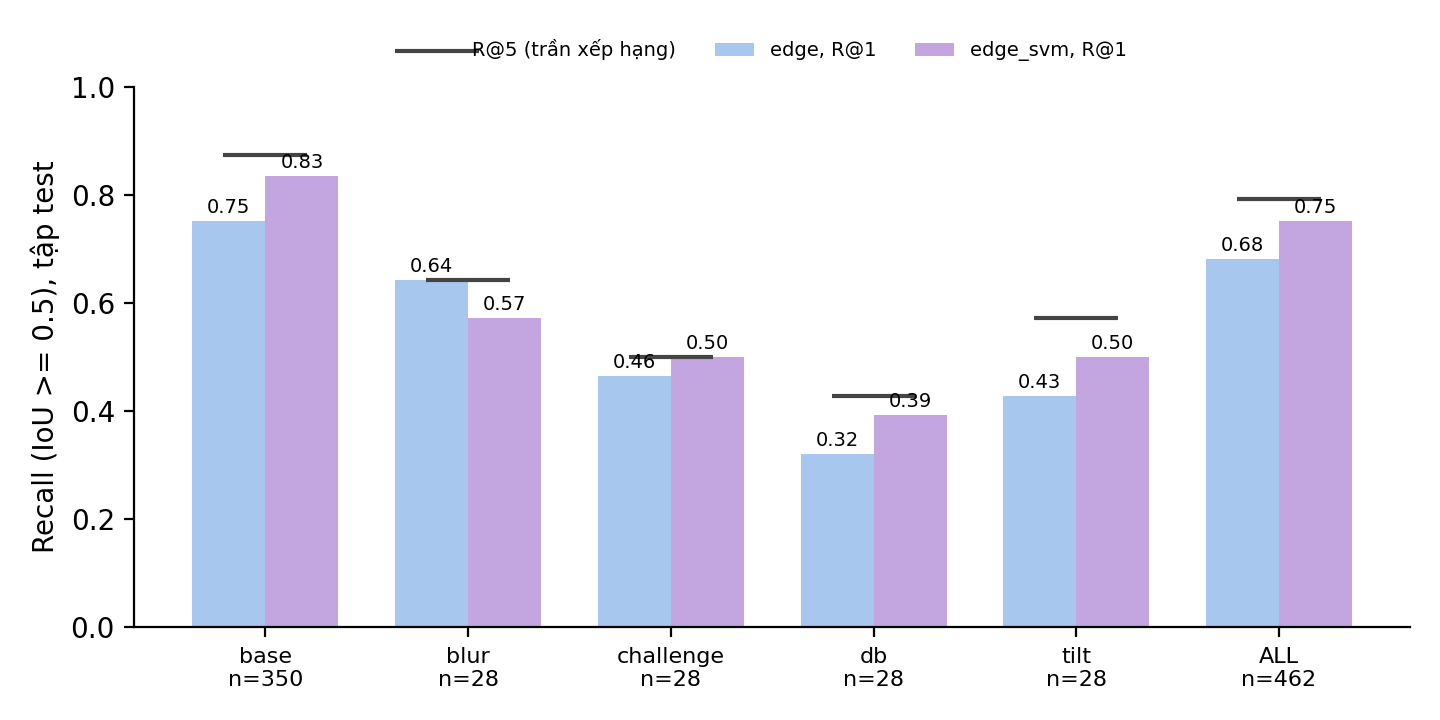
\includegraphics[width=0.85\textwidth]{figures/e3_subset_r1.png}
\caption[Recall@1 của edge và edge\_svm theo nhóm (test)]{Recall@1 của \code{edge} và \code{edge\_svm} theo nhóm (test). Vạch đen là Recall@5, trần mà bước xếp hạng không vượt qua được. Nguồn: \code{e3\_localization.csv}.}
\label{fig:e3}
\end{figure}

Trên toàn test, top-1 của \code{edge\_svm} đạt $0.751$ so với $0.682$ của \code{edge} (tune: $0.803$ so với $0.747$; số tune của SVM lạc quan vì mô hình huấn luyện trên chính tập này). Mức tăng $+6.9$ điểm trên test tương ứng $+32$ ảnh trúng (315 $\to$ 347): \code{base} $+29$, \code{challenge} $+1$, \code{db} $+2$, \code{tilt} $+2$, \code{blur} $-2$. SVM không thêm ứng viên nên Recall@5 của hai phương pháp bằng nhau (0.792 trên test); toàn bộ cải thiện nằm ở Recall@1, và \code{edge\_svm} còn cách trần Recall@5 khoảng 4 điểm. Khoảng 21\% ảnh test không có ứng viên đúng trong top-5 (riêng \code{db} 57\%, \code{challenge} 50\%, \code{tilt} 43\%), nên muốn tăng tiếp thì phải cải thiện khâu sinh ứng viên, không phải khâu xếp hạng. SVM thêm 4.8 ms/ảnh trong E7 (sổ thí nghiệm ghi khoảng 14 ms khi máy đang tải).

\section{Nắn biển: cắt bbox so với warp quad (E4)}
\label{sec:e4}

E4 chạy toàn pipeline (định vị \code{edge\_svm} + bilateral, nhị phân Otsu, tách ký tự CCA của B) trên test, thay đổi duy nhất là cách lấy ảnh biển $220\times 70$: cắt bbox hay warp quad. Bảng~\ref{tab:e4} báo ba nguồn crop; Bảng~\ref{tab:e4sub} tách theo nhóm cho các ảnh top-1 đúng.

\begin{table}[htbp]
\centering
\caption[E4: cắt bbox so với warp quad (test, ALL)]{E4: cắt bbox so với warp quad, tập test, dòng ALL. Sai số góc tính theo pixel ảnh gốc trên 347 ảnh top-1 đúng. Nguồn: \code{e4\_rectify.csv}.}
\label{tab:e4}
\footnotesize
\setlength{\tabcolsep}{3pt}
\rowcolors{2}{white}{tablerowalt}
\arrayrulecolor{tableheader}
\begin{tabularx}{\textwidth}{llCCCCCC}
\hline
\rowcolor{tableheader} \tblhd{Nguồn crop} & \tblhd{Crop} & \tblhd{$n$} & \tblhd{corner (tb / trung vị)} & \tblhd{count\_\allowbreak match} & \tblhd{pos0} & \tblhd{pos1--6} & \tblhd{all\_\allowbreak correct} \\
\hline
gt & bbox & 462 & -- & 0.452 & 0.571 & 0.597 & 0.262 \\
gt & quad & 462 & -- & 0.606 & 0.805 & 0.815 & 0.563 \\
\hline
pred & bbox & 462 & 25.2 / 19.4 & 0.262 & 0.266 & 0.391 & 0.093 \\
pred & quad & 462 & 16.3 / 13.8 & 0.400 & 0.496 & 0.518 & 0.195 \\
\hline
pred\_tp & bbox & 347 & 25.2 / 19.4 & 0.346 & 0.329 & 0.498 & 0.124 \\
pred\_tp & quad & 347 & 16.3 / 13.8 & 0.513 & 0.625 & 0.641 & 0.259 \\
\hline
\end{tabularx}
\end{table}


\begin{tabular}{lrrrrrrr}
\toprule
Nhóm & $n$ & corner bbox & corner quad & count bbox & count quad & all bbox & all quad \\
\midrule
base & 292 & 23.0 & 15.3 & 0.387 & 0.558 & 0.130 & 0.291 \\
blur & 16 & 22.8 & 16.0 & 0.125 & 0.062 & 0.125 & 0.000 \\
challenge & 14 & 23.7 & 19.2 & 0.143 & 0.214 & 0.000 & 0.143 \\
db & 11 & 34.7 & 24.0 & 0.273 & 0.455 & 0.273 & 0.273 \\
tilt & 14 & 68.0 & 28.9 & 0.000 & 0.429 & 0.000 & 0.000 \\
ALL & 347 & 25.2 & 16.3 & 0.346 & 0.513 & 0.124 & 0.259 \\
\bottomrule
\end{tabular}


Warp quad thắng cắt bbox ở mọi cột trên ALL: sai số góc giảm từ $25.2$ xuống $16.3$ px (trung vị $19.4\to 13.8$), \code{all\_correct} trên các ảnh top-1 đúng tăng từ $0.124$ lên $0.259$. Khi cô lập hẳn khỏi lỗi định vị (crop \code{gt}), \code{all\_correct} tăng từ $0.262$ lên $0.563$, tức phép nắn tự nó đã làm \code{all\_correct} tăng hơn gấp đôi. Nhóm \code{tilt} cho thấy đúng lý do: bbox ngang không bù được độ nghiêng, sai số góc $68.0$ px so với $28.9$ px của quad và \code{count\_match} $0.000$ so với $0.429$.

\textbf{Ngoại lệ ở nhóm \code{blur}} ($n=16$ ảnh top-1 đúng): bbox nhỉnh hơn quad ở \code{all\_correct} ($0.125$ so với $0.000$), \code{count\_match} ($0.125$ so với $0.063$) và \code{pos1\textendash 6} ($0.240$ so với $0.229$), dù sai số góc của quad vẫn tốt hơn ($16.0$ so với $22.8$ px). Chênh lệch này là 1--2 ảnh (một ảnh bằng $0.063$) nên chưa kết luận được. Nhóm \code{tilt} hòa ở \code{all\_correct} (cùng bằng 0) vì cả hai cách đều hỏng hết.

Có hai cảnh báo. Thứ nhất, lợi ích của \code{approxpoly} so với \code{minarearect} nhỏ: trên 128 ảnh tune có top-1 đúng (cấu hình định vị giai đoạn đầu), sai số góc trung bình chỉ giảm từ $19.7$ xuống $17.6$ px; theo từng ảnh có 45 ảnh tốt hơn, 48 kém hơn, 35 hòa (Wilcoxon $p=0.46$), nên khác biệt này không có ý nghĩa thống kê, và hằng số được chỉnh trên đúng tập đó. Lợi ích lớn ở E4 chủ yếu đến từ việc dùng quad nghiêng thay vì bbox ngang. Thứ hai, ở crop \code{gt} và \code{pred\_tp} có khoảng cách lớn ($0.563$ so với $0.259$ ở \code{all\_correct} của warp quad): dù IoU $\ge 0.5$, quad dự đoán vẫn lệch trung bình khoảng 16 px so với quad thật. Chúng tôi \emph{giả thuyết} độ lệch này là nguyên nhân chính khiến khoảng một nửa số biển hỏng ở bước tách ký tự; bảng chéo (Bảng~\ref{tab:cross}) chỉ xác nhận một phần: trong 257 ảnh top-1 đúng nhưng vẫn lỗi, 152 ảnh tách đúng khi crop \code{gt}, nên lỗi nằm ở crop dự đoán, còn phần do quad lệch cụ thể thì chưa tách riêng được. Trong 128 ảnh tune nói trên, 107 ảnh có ít nhất một góc thật nằm ngoài quad ứng viên, nên trần sai số do bước định vị quyết định, không phải bước tinh chỉnh quad.

\section{Thời gian chạy từng bước (E7)}
\label{sec:e7}

E7 đo thời gian từng bước của pipeline đầy đủ trên test (Bảng~\ref{tab:e7}), một tiến trình, ms/ảnh.

\begin{table}[htbp]
\centering
\caption[E7: thời gian từng bước (test, ALL)]{E7: thời gian từng bước, tập test, dòng ALL (ms/ảnh). Nguồn: \code{e7\_runtime.csv}. Bước ``Sobel, morph, lọc, NMS'' được ước lượng bằng hiệu thời gian \code{localize\_edge} trừ thời gian tiền xử lý đo riêng. 30 ảnh không có ứng viên nên các bước sau định vị chỉ có $n=432$.}
\label{tab:e7}
\small
\rowcolors{2}{white}{tablerowalt}
\arrayrulecolor{tableheader}
\begin{tabularx}{\textwidth}{lCCC}
\hline
\rowcolor{tableheader} \tblhd{Bước} & \tblhd{$n$} & \tblhd{tb (ms)} & \tblhd{p95 (ms)} \\
\hline
tiền xử lý (resize, xám, CLAHE, lọc) & 462 & 69.79 & 134.32 \\
Sobel, morph đa tỉ lệ, lọc, NMS (ước lượng) & 462 & 63.50 & 149.30 \\
HOG + SVM & 462 & 4.77 & 10.77 \\
ước lượng quad & 432 & 0.97 & 2.20 \\
warp 220$\times$70 & 432 & 0.34 & 0.59 \\
nhị phân hóa (B) & 432 & 0.10 & 0.18 \\
tách ký tự (B) & 432 & 0.43 & 0.76 \\
\hline
\textbf{tổng (không SVM)} & 462 & 135.01 & 247.69 \\
\textbf{tổng} & 462 & 139.79 & 262.16 \\
\hline
\end{tabularx}
\end{table}


Tổng thời gian trung bình là 139.8 ms/ảnh (p95 262.2 ms). Định vị chiếm gần như toàn bộ: tiền xử lý khoảng 50\% (69.8 ms, phần lớn là bilateral đường kính 11 trên ảnh 800 px), Sobel cùng morph đa tỉ lệ khoảng 45\% (63.5 ms), SVM khoảng 3\% (4.8 ms). Các bước nắn, nhị phân hóa và tách ký tự cộng lại chỉ 1.8 ms. Theo nhóm, \code{tilt} chậm nhất (208.4 ms) và \code{challenge} nhanh nhất (88.5 ms; \code{db} 92.6 ms). Số tuyệt đối trong lần đo ghi trong sổ thí nghiệm cao hơn nhiều (416 ms/ảnh) vì máy khi đó đang chạy nhiều tiến trình; tỉ lệ giữa các bước cũng dịch theo tải máy (tiền xử lý 44\% $\to$ 50\%, Sobel cùng morph 51\% $\to$ 45\%, SVM 3.3\% $\to$ 3.4\%), nên chỉ xem tỉ lệ là gần đúng. Nếu cần số tuyệt đối cho kết luận về tốc độ thì nên đo lại trên máy riêng.

\chapter{PHÂN TÍCH LỖI VÀ THẢO LUẬN}
\label{chap:a-discussion}

\section{Triage lỗi theo bước pipeline}
\label{sec:triage}

Để biết pipeline mất ảnh ở đâu, mỗi ảnh test được gán đúng một \emph{bước lỗi chính}, xét theo thứ tự pipeline. Cấu hình: định vị \code{edge\_svm} + bilateral, crop quad, nhị phân Otsu, tách ký tự CCA (như E4). Bảng~\ref{tab:stagedef} định nghĩa các bước; kết quả đếm ở Bảng~\ref{tab:triage} và Hình~\ref{fig:triage}.

\begin{table}[htbp]
\centering
\caption{Định nghĩa bước lỗi chính (ưu tiên từ trên xuống).}
\label{tab:stagedef}
\small
\rowcolors{2}{white}{tablerowalt}
\arrayrulecolor{tableheader}
\begin{tabularx}{\textwidth}{lY}
\hline
\rowcolor{tableheader} \tblhd{Bước} & \tblhd{Điều kiện} \\
\hline
\code{loc\_no\_candidate} & không ứng viên nào trong top-5 có IoU $\ge 0.5$ với bbox thật \\
\code{loc\_rank} & có ứng viên đúng trong top-5 nhưng không phải top-1 \\
\code{rectify} & top-1 đúng, không \code{all\_correct}, và sai số góc quad lớn hơn ngưỡng \\
\code{segment\_count} & top-1 đúng, nắn ổn, nhưng số hộp ký tự khác 7 \\
\code{segment\_position} & đủ 7 hộp nhưng có vị trí không trúng khuôn \\
\code{ok} & top-1 đúng và \code{all\_correct} \\
\hline
\end{tabularx}
\end{table}

Ngưỡng sai số góc là $22.30$ px, bằng phân vị 95 của sai số góc trên tune trong số ảnh top-1 đúng và tách đúng hết ($n=50$ trong 159 ảnh top-1 đúng; trung vị 10.84 px, trong khi nhóm top-1 đúng nhưng tách sai có trung vị 19.84 px). Nói cách khác, đó là mức sai số mà ảnh tách tốt còn chịu được. Ngưỡng tính bằng pixel của ảnh gốc nên phụ thuộc kích thước biển trong ảnh. Ngưỡng chọn trên tune, không dùng số test. Ảnh nắn lệch nhưng vẫn tách đúng thì là \code{ok}; ảnh top-1 sai không bao giờ là \code{ok}.

\begin{table}[htbp]
\centering
\caption[Số ảnh test theo bước lỗi chính và nhóm]{Số ảnh test theo bước lỗi chính và nhóm (trong ngoặc là số ảnh của nhóm); cột cuối là phần trăm trên toàn test ($n=462$). Nguồn: \code{triage\_stage\_counts.csv}.}
\label{tab:triage}
\footnotesize
\setlength{\tabcolsep}{3pt}
\rowcolors{2}{white}{tablerowalt}
\arrayrulecolor{tableheader}
\begin{tabularx}{\textwidth}{lCCCCCCC}
\hline
\rowcolor{tableheader} \tblhd{Bước} & \tblhd{base (350)} & \tblhd{blur (28)} & \tblhd{challenge (28)} & \tblhd{db (28)} & \tblhd{tilt (28)} & \tblhd{ALL (462)} & \tblhd{\% ALL} \\
\hline
loc\_no\_candidate & 44 & 10 & 14 & 16 & 12 & 96 & 20.8 \\
loc\_rank & 14 & 2 & 0 & 1 & 2 & 19 & 4.1 \\
rectify & 40 & 4 & 4 & 2 & 9 & 59 & 12.8 \\
segment\_count & 100 & 11 & 7 & 4 & 1 & 123 & 26.6 \\
segment\_position & 67 & 1 & 1 & 2 & 4 & 75 & 16.2 \\
ok & 85 & 0 & 2 & 3 & 0 & 90 & 19.5 \\
\hline
\end{tabularx}
\end{table}


Kiểm tra chéo với E3 và E6: \code{ok} $=90=0.1948\times 462$, khớp \code{all\_correct} của crop \code{pred} quad ở E4 và của tách \code{cca} với crop \code{pred} ở E6 (cả hai đều 0.1948); \code{loc\_no\_candidate} $+$ \code{loc\_rank} $=115=462-347$, khớp số ảnh top-1 sai của \code{edge\_svm}.

\begin{figure}[htbp]
\centering
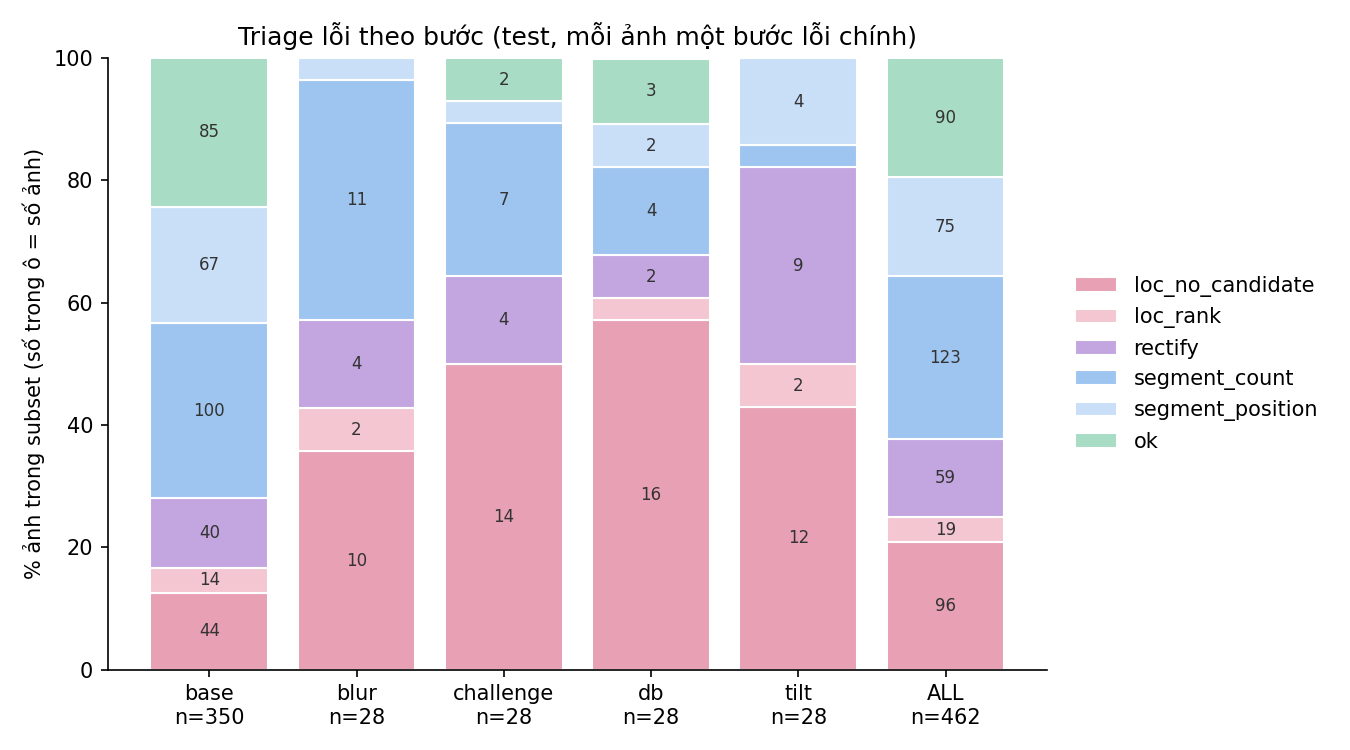
\includegraphics[width=0.85\textwidth]{figures/triage_stages.png}
\caption[Phân bố bước lỗi chính theo nhóm (test)]{Phân bố bước lỗi chính theo nhóm (test); số trong ô là số ảnh. Nguồn: \code{triage\_stage\_counts.csv}.}
\label{fig:triage}
\end{figure}

\textbf{Đọc bảng.} Theo Bảng~\ref{tab:triage} (và Hình~\ref{fig:triage}), chỉ 19.5\% ảnh test đi hết pipeline đúng. Lỗi lớn nhất là tách ký tự (\code{segment\_count} 26.6\% và \code{segment\_position} 16.2\%, tổng 42.8\%), kế đến là định vị (\code{loc\_no\_candidate} 20.8\% và \code{loc\_rank} 4.1\%, tổng 24.9\%) và nắn (12.8\%). Hai kiểu lỗi định vị rất khác nhau: \code{loc\_rank} (19 ảnh) là lỗi xếp hạng, \code{loc\_no\_candidate} (96 ảnh) là lỗi sinh ứng viên và lớn gấp năm lần. Trong 96 ảnh đó, 30 ảnh không có ứng viên nào và 66 ảnh có ứng viên nhưng đều IoU $<0.5$; chỉ 12 ảnh có bbox thật nhỏ hơn cận dưới \code{area\_ratio} (3 \code{base}, 1 \code{blur}, 7 \code{challenge}, 1 \code{db}), còn 84 ảnh thuộc nhóm ``khác'', nghĩa là bộ lọc diện tích chỉ giải thích được một phần nhỏ. Các nhóm khó gần như không có ảnh \code{ok} (0--3 trên 28 ảnh) và mất chủ yếu ở định vị (\code{loc\_no\_candidate} từ 36\% đến 57\%) và nắn (riêng \code{tilt}: 9/28 ảnh \code{rectify}), trừ \code{blur}: ở nhóm này định vị (12 ảnh) và tách ký tự (12 ảnh) mất bằng nhau. Nhóm \code{base} mất nhiều nhất ở tách ký tự (167/350 ảnh).

\textbf{Bảng chéo crop \code{gt} và crop \code{pred}.} Để phân biệt lỗi do định vị/nắn với lỗi do bộ tách ký tự, Bảng~\ref{tab:cross} đếm số ảnh theo trạng thái tách khi crop từ bbox/quad thật (hàng) và bước lỗi khi crop từ dự đoán (cột).

\begin{tabular}{lrrrrrr}
\toprule
crop gt $\backslash$ bước pred & loc\_no\_candidate & loc\_rank & rectify & segment\_count & segment\_position & ok \\
\midrule
ok (260) & 34 & 8 & 32 & 64 & 56 & 66 \\
segment\_count (182) & 57 & 8 & 21 & 57 & 15 & 24 \\
segment\_position (20) & 5 & 3 & 6 & 2 & 4 & 0 \\
\bottomrule
\end{tabular}


Trong 257 ảnh top-1 đúng nhưng vẫn lỗi (\code{rectify} $+$ \code{segment}), 152 ảnh tách đúng khi crop \code{gt}, tức lỗi do crop dự đoán (nắn lệch hoặc bbox không khít); 105 ảnh tách sai ngay cả với crop \code{gt}, tức lỗi do bộ tách. Hai nguồn này cùng bậc, nên cải thiện định vị/nắn và cải thiện bộ tách ký tự đều cần thiết. Còn 42 ảnh tách đúng ở crop \code{gt} nhưng hỏng ở định vị (34 \code{loc\_no\_candidate}, 8 \code{loc\_rank}) là lỗi thuần của định vị. Có 24 ảnh (trong 202 ảnh crop \code{gt} lỗi, khoảng 12\%) crop \code{gt} tách sai nhưng crop \code{pred} lại \code{ok}: viền cắt khác nên ký tự không dính, tức crop dự đoán tình cờ tốt hơn crop thật; tỉ lệ này không nhỏ.

\section{Quan sát định tính}
\label{sec:qual}

Hình~\ref{fig:grids} cho một ví dụ cho mỗi bước lỗi, trích từ các lưới gỡ lỗi (ứng viên đỏ và bbox thật xanh, mặt nạ morph, crop dự đoán và crop \code{gt} cùng ảnh nhị phân và hộp ký tự). Mỗi bước chọn 12 ảnh theo seed 42 để đọc; dưới đây là các quan sát từ lưới đó và từ bảng đếm.

\begin{figure}[htbp]
\centering
\begin{subfigure}[t]{0.48\textwidth}
  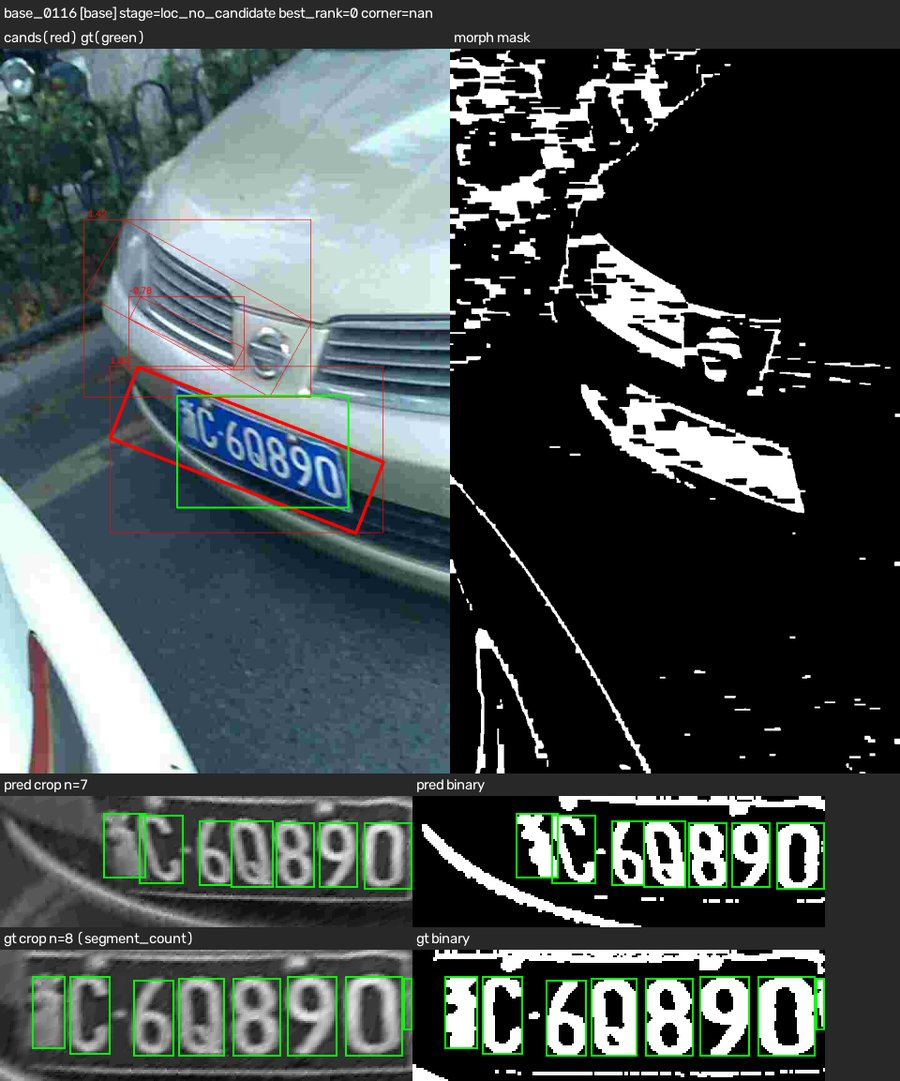
\includegraphics[width=\textwidth,height=0.255\textheight,keepaspectratio]{figures/grid_loc_no_candidate.jpg}
  \caption{\code{loc\_no\_candidate}}
\end{subfigure}\hfill
\begin{subfigure}[t]{0.48\textwidth}
  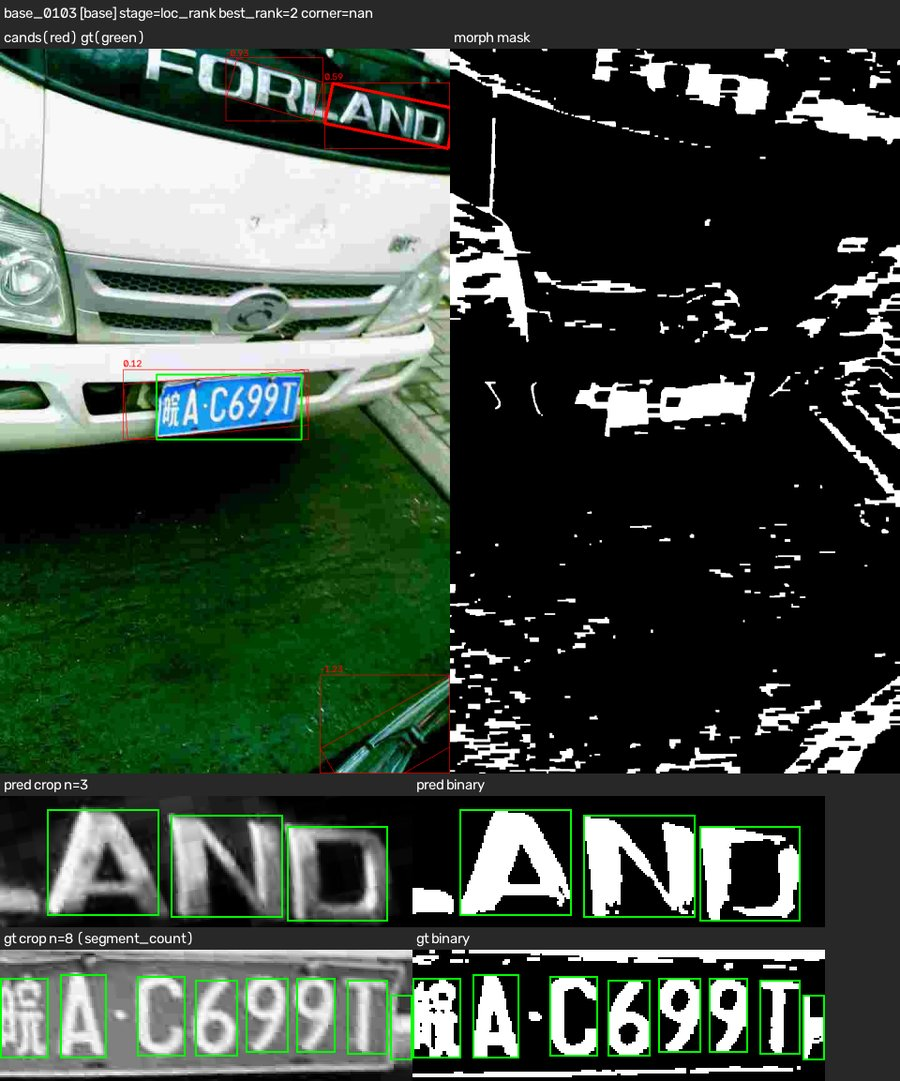
\includegraphics[width=\textwidth,height=0.255\textheight,keepaspectratio]{figures/grid_loc_rank.jpg}
  \caption{\code{loc\_rank}}
\end{subfigure}

\medskip
\begin{subfigure}[t]{0.48\textwidth}
  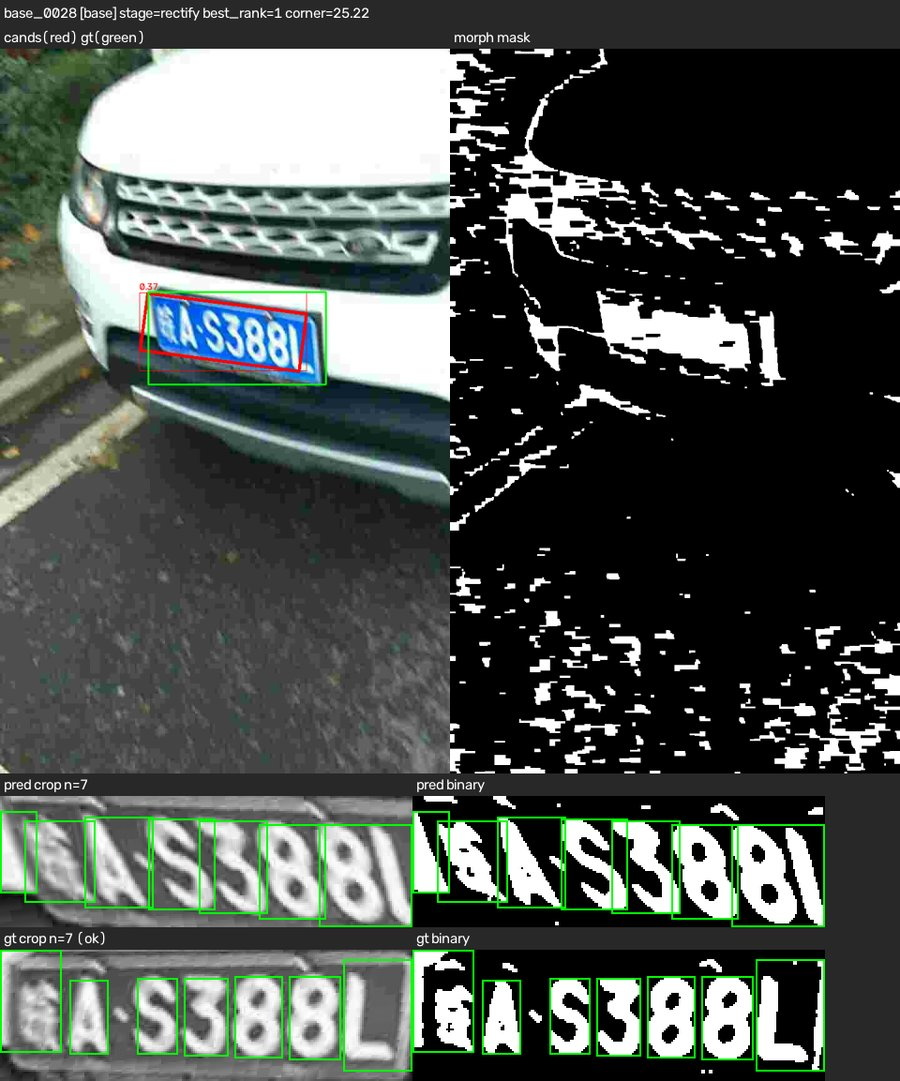
\includegraphics[width=\textwidth,height=0.255\textheight,keepaspectratio]{figures/grid_rectify.jpg}
  \caption{\code{rectify}}
\end{subfigure}\hfill
\begin{subfigure}[t]{0.48\textwidth}
  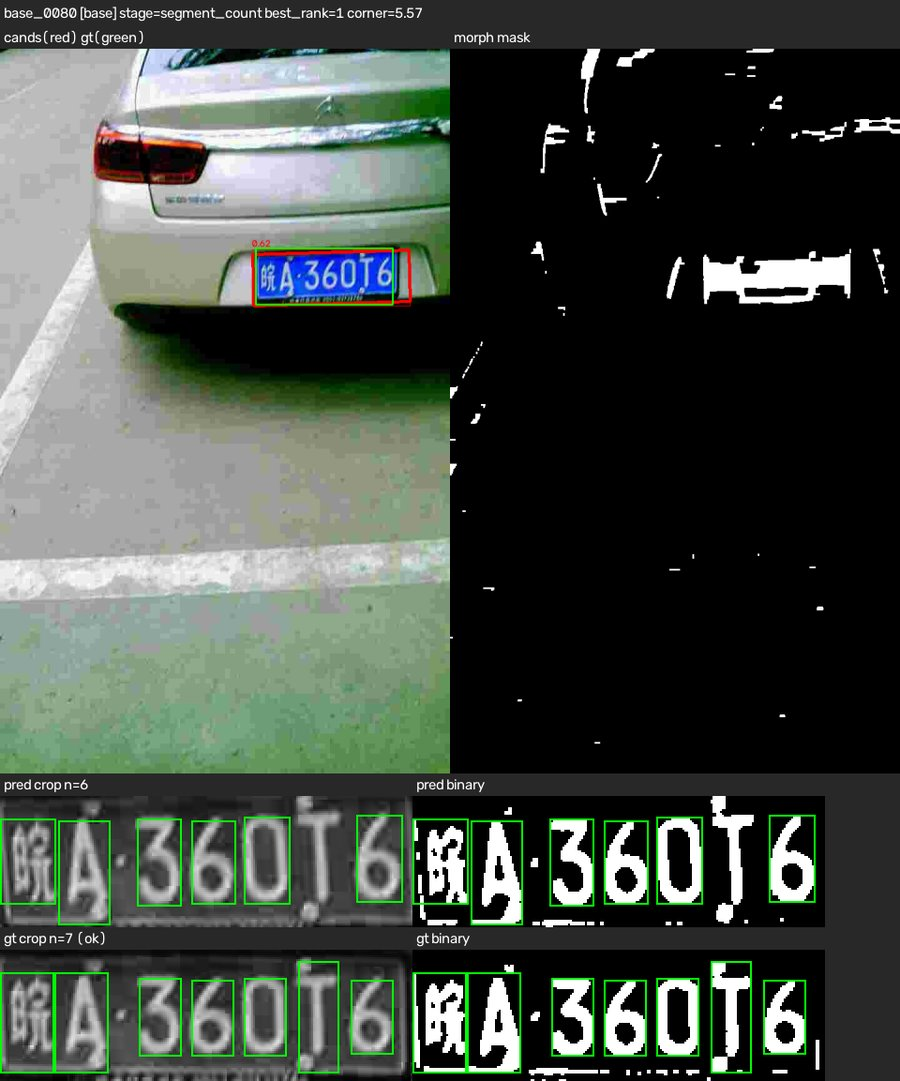
\includegraphics[width=\textwidth,height=0.255\textheight,keepaspectratio]{figures/grid_segment_count.jpg}
  \caption{\code{segment\_count}}
\end{subfigure}

\medskip
\begin{subfigure}[t]{0.48\textwidth}
  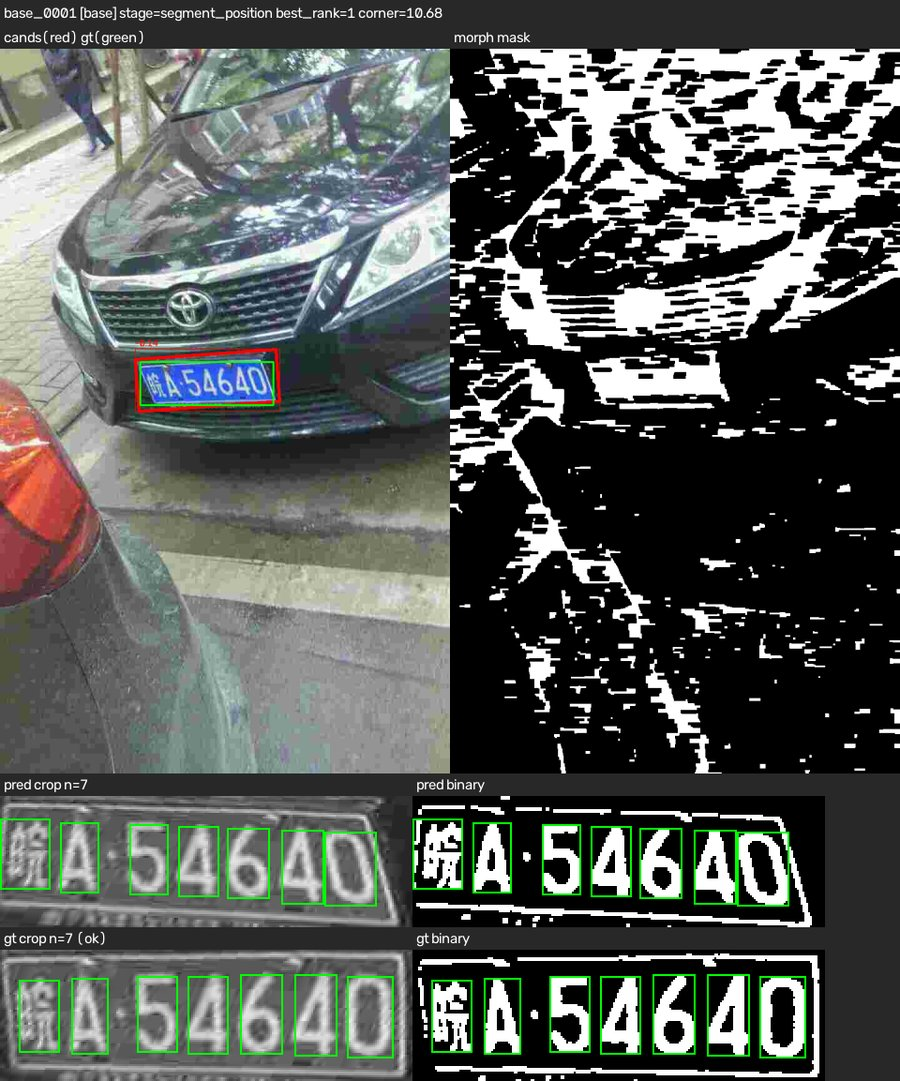
\includegraphics[width=\textwidth,height=0.255\textheight,keepaspectratio]{figures/grid_segment_position.jpg}
  \caption{\code{segment\_position}}
\end{subfigure}
\caption[Mỗi bước lỗi một ví dụ (test)]{Mỗi bước lỗi một ví dụ trên tập test (ảnh \code{base\_0116}, \code{base\_0103}, \code{base\_0028}, \code{base\_0080}, \code{base\_0001}). Hình gốc có độ phân giải cao hơn, có thể phóng to trong bản PDF.}
\label{fig:grids}
\end{figure}

\begin{itemize}
  \item \textbf{\code{loc\_no\_candidate}.} Ba dạng thường gặp: (1) ứng viên top-1 bao cả biển lẫn phần thân xe hoặc khung nên IoU thấp dù nhìn bằng mắt là trúng; biển nghiêng bị bbox ngang phạt nặng; (2) biển dính vào lưới tản nhiệt hoặc cản xe nên vùng sau morph không tách ra; (3) ảnh \code{challenge} nắng gắt, nhợt màu: mặt nạ morph phủ cả nền nhà và biển chỉ được điểm rất thấp (khoảng 0.01). Có 47/96 ảnh mà crop dự đoán không cho hộp ký tự nào.
  \item \textbf{\code{loc\_rank}.} 18 trong 19 ảnh có biển đúng ở hạng 2. Top-1 thường là chữ hãng xe hoặc logo ở đầu xe, có cạnh đứng dày (ví dụ chữ ``FORLAND'' trong Hình~\ref{fig:grids}b), mà SVM cho điểm cao hơn biển thật. Điều này gợi ý SVM chưa học đủ mẫu âm dạng chữ lớn trên nền tối.
  \item \textbf{\code{rectify}.} Warp thường cắt cụt hoặc làm lệch biển nên crop thiếu ký tự: trong 59 ảnh nhóm này, số hộp ký tự dự đoán là 0 (8 ảnh), 1 (4), 2 (1), 3 (1), 4 (5), 5 (13), 6 (9), 7 (13), 8 (4), 9 (1); chỉ 5/59 ảnh có 8--9 hộp và 41/59 có không quá 6 hộp (trung bình 4.75). Sai số góc trung bình của nhóm này là 34.9 px (so với 10.8 px của nhóm \code{ok}). Nhóm này nằm nhiều ở \code{tilt} (9/28) và \code{base}.
  \item \textbf{\code{segment\_count}.} Chủ yếu 6 hộp (54/123 ảnh) do ký tự Hán dính ký tự A (cả crop \code{gt} cũng bị), và 8 hộp (27/123) do mảnh nền hoặc khung biển ở mép; 64/123 ảnh này tách đúng trên crop \code{gt}.
  \item \textbf{\code{segment\_position}.} Đủ 7 hộp nhưng lệch khuôn vài pixel, thường ở ký tự Hán (nét rời, dính A), chữ số ``1'' hẹp và ký tự cuối chạm viền; crop dự đoán hơi lệch hoặc co làm cả dãy hộp trượt khỏi khuôn.
  \item {\sloppy \textbf{Theo mức nghiêng và mờ.} Mã hóa CCPD cho góc nghiêng ngang/dọc và độ mờ; chỉ dùng so sánh tương đối. Trung bình, ảnh \code{ok} có giá trị nghiêng cao nhất (86 và 82) so với \code{loc\_no\_candidate} (48 và 47) và \code{rectify} (66 và 63); độ mờ trung bình 58 ở \code{ok} so với 45 ở \code{loc\_no\_candidate}. Các giá trị này theo quy ước mã hóa của CCPD nên không nên hiểu là góc thật hay độ mờ thật.\par}
\end{itemize}

\section{Hạn chế}
\label{sec:limits}

\begin{itemize}
  \item \textbf{Cận diện tích của bộ lọc.} Trên test, 16/462 bbox thật nhỏ hơn cận dưới \code{area\_ratio} 0.008 (và 1 bbox lớn hơn 0.16). Đây không phải trần cứng: bộ lọc xét diện tích \code{minAreaRect} của ứng viên và IoU $\ge 0.5$ cho phép ứng viên lớn hơn bbox thật. Triage cho thấy chỉ 12/16 bbox nhỏ bị mất ở định vị (4 ảnh còn lại không mất ở đó), còn bbox lớn duy nhất (0.182) là lỗi xếp hạng \code{loc\_rank}.
  \item \textbf{IoU trục ngang phạt biển nghiêng.} Độ đo IoU dùng bbox ngang, nên biển nghiêng bị chấm thấp dù ứng viên bám đúng biển; điều này góp phần vào \code{loc\_no\_candidate}. Chưa dùng IoU của đa giác nghiêng.
  \item \textbf{Thời gian đo trên máy không rảnh.} Lần chạy dùng trong báo cáo (khoảng 140 ms/ảnh) đo trên máy ít tải hơn lần ghi trong sổ (416 ms/ảnh) nhưng vẫn không phải máy chuyên dụng. Tỉ lệ giữa các bước cũng dịch theo tải máy (tiền xử lý 44\% $\to$ 50\%, Sobel cùng morph 51\% $\to$ 45\%), nên chỉ xem là gần đúng; số đo lại ghi ở mục ``Đo lại thời gian (máy ít tải)'' trong \code{notes.md}.
  \item \textbf{Rò rỉ nhẹ ở kiểm chứng chéo của SVM.} Chia fold theo patch chứ không theo ảnh, nên số CV (F1 0.919) lạc quan; số định vị trên test mới phản ánh chất lượng thực. Số tune của \code{edge\_svm} cũng lạc quan vì huấn luyện trên chính tune.
  \item \textbf{Các nhóm khó rất nhỏ.} Mỗi nhóm \code{blur}, \code{db}, \code{challenge}, \code{tilt} chỉ 28 ảnh test (12 ảnh tune); một ảnh là 0.036, nên các so sánh (kể cả ngoại lệ \code{blur} ở E4) có độ bất định lớn. Chúng tôi chưa tính khoảng tin cậy và chỉ có một lần chia tune/test.
  \item \textbf{Một số lựa chọn dựa trên tune nhỏ.} Việc chọn \code{approxpoly} dựa trên 128 ảnh tune và khác biệt không có ý nghĩa thống kê; ngưỡng triage 22.3 px dựa trên 50 ảnh.
\end{itemize}

\section{Hướng cải thiện}

Vì 21\% ảnh test không có ứng viên đúng trong top-5, ưu tiên là bổ sung khâu sinh ứng viên, ví dụ thêm nguồn ứng viên theo màu biển hoặc bù nghiêng trước bước morph (chưa thử). Ở khâu xếp hạng, có thể thêm mẫu âm khó (chữ hãng xe, logo) vào SVM và chia fold theo ảnh khi kiểm chứng. Ở khâu nắn, cần quad chính xác hơn vì sai số khoảng 16 px nhiều khả năng góp phần đáng kể vào lỗi (giả thuyết; 152/257 ảnh top-1 đúng nhưng lỗi tách đúng khi crop \code{gt}); và dùng IoU đa giác để đánh giá công bằng hơn với biển nghiêng. Lỗi dính ký tự Hán với chữ A thuộc phần tách ký tự và được nêu ở phần của B.

\chapter{PHẦN CỦA THÀNH VIÊN B: HỆ MÀU, NHỊ PHÂN HÓA, TÁCH KÝ TỰ}
\label{chap:b}

\TODO{Chương này là chỗ dành sẵn cho thành viên B (\TenB); nội dung chưa được viết.}

\section{Phân tích hệ màu (E1)}
\label{sec:b-color}

\TODO{Phần của Bích}

\section{Nhị phân hóa: Otsu và adaptive (E5)}
\label{sec:b-binarize}

\TODO{Phần của Bích}

\section{Tách ký tự: CCA và projection (E6)}
\label{sec:b-segment}

\TODO{Phần của Bích}

\section{Ảnh biển số Việt Nam tự chụp, đánh giá định tính (E8)}
\label{sec:b-vn}

\TODO{Phần của Bích}

\chapter{KẾT LUẬN}
\label{chap:conclusion}

Báo cáo trình bày phần A của dự án: tiền xử lý, định vị biển số bằng cạnh và hình thái học (có xếp hạng lại bằng HOG và SVM tuyến tính), nắn phối cảnh, và triage lỗi theo bước pipeline, trên tập con 660 ảnh CCPD2019 chia thành tune (198 ảnh) và test (462 ảnh).

Các kết quả chính trên tập test, ngưỡng IoU $\geq 0.5$:
\begin{itemize}
  \item Bộ lọc bilateral được chọn trên tune và cho F1 định vị cao hơn rõ rệt so với ba bộ lọc còn lại (0.705 so với 0.592--0.630 trên test).
  \item Sau khi tinh chỉnh bước định vị (Issue \#10), Recall@1 của \code{edge} tăng từ 0.545 lên 0.682 và \code{cand\_recall} từ 0.667 lên 0.792. Xếp hạng lại bằng SVM nâng Recall@1 lên 0.751 (315 $\to$ 347 ảnh trúng); Recall@5 giữ nguyên 0.792, nên còn khoảng 21\% ảnh không có ứng viên đúng trong top-5.
  \item Nắn bằng warp quad tốt hơn cắt bbox ở mọi cột trên ALL: sai số góc giảm từ 25.2 xuống 16.3 px, và \code{all\_correct} trên các ảnh top-1 đúng tăng từ 0.124 lên 0.259 (crop \code{gt}: 0.262 lên 0.563).
  \item Triage: chỉ 19.5\% ảnh test đi hết pipeline đúng (90/462). Lỗi lớn nhất là tách ký tự (42.8\%), kế đến là định vị (24.9\%) và nắn (12.8\%).
  \item Thời gian trung bình 139.8 ms/ảnh, trong đó định vị chiếm gần như toàn bộ.
\end{itemize}

Các hạn chế chính: các nhóm khó chỉ có 28 ảnh test nên so sánh giữa các nhóm có độ bất định lớn; số CV và số tune của SVM lạc quan; lợi ích của \code{approxpoly} so với \code{minarearect} không có ý nghĩa thống kê; thời gian đo trên máy không chuyên dụng. Hướng cải thiện ưu tiên là bổ sung khâu sinh ứng viên (theo màu biển hoặc bù nghiêng trước bước morph, chưa thử), thêm mẫu âm khó cho SVM, nắn chính xác hơn, và dùng IoU đa giác (mục~\ref{sec:limits} và phần hướng cải thiện ở Chương~\ref{chap:a-discussion}).

\TODO{Kết luận chung của cả nhóm sau khi có phần của Bích (Chương~\ref{chap:b})}


\chapter*{TÀI LIỆU THAM KHẢO}
\addcontentsline{toc}{chapter}{Tài liệu tham khảo}
\begin{thebibliography}{99}

\bibitem{ccpd}
Xu, Z., Yang, W., Meng, A., Lu, N., Huang, H., Ying, C., Huang, L. (2018). Towards End-to-End License Plate Detection and Recognition: A Large Dataset and Baseline. \textit{European Conference on Computer Vision (ECCV)}.

\bibitem{otsu}
Otsu, N. (1979). A threshold selection method from gray-level histograms. \textit{IEEE Transactions on Systems, Man, and Cybernetics}, 9(1), 62--66.

\bibitem{hog}
Dalal, N., Triggs, B. (2005). Histograms of oriented gradients for human detection. \textit{IEEE Conference on Computer Vision and Pattern Recognition (CVPR)}, 886--893.

\bibitem{svm}
Cortes, C., Vapnik, V. (1995). Support-vector networks. \textit{Machine Learning}, 20(3), 273--297.

\bibitem{bilateral}
Tomasi, C., Manduchi, R. (1998). Bilateral filtering for gray and color images. \textit{IEEE International Conference on Computer Vision (ICCV)}, 839--846.

\bibitem{clahe}
Zuiderveld, K. (1994). Contrast limited adaptive histogram equalization. In \textit{Graphics Gems IV}, Academic Press, 474--485.
\end{thebibliography}

\end{document}
